\documentclass[a4paper,11pt]{book}

\usepackage[utf8]{inputenc}
\usepackage[T1]{fontenc}
\usepackage{lmodern}
\usepackage[headings]{fullpage}
\usepackage{color}
\usepackage[dvipsnames]{xcolor}
\usepackage[outline]{contour}
\usepackage{ifthen}
\usepackage{import}
\usepackage{graphicx}
\usepackage{amsfonts}
\usepackage{amsmath}
\usepackage{bm}
\usepackage{tikz}
\usetikzlibrary{arrows.meta}
\usetikzlibrary{decorations.markings}
%\usepackage{todonotes}

\definecolor{dgreen}{rgb}{0,0.6,0}
\usepackage[colorlinks=true,citecolor=dgreen]{hyperref}

\newboolean{french}
\setboolean{french}{false}

\newboolean{warnings}
\setboolean{warnings}{false}

\usepackage{inconsolata}

\newcommand{\dsp}{\displaystyle}
%\newcommand{\langswitch}[2]{\ifthenelse{\boolean{french}}{#1}{#2}}

\newcommand{\fwarn}{\ifthenelse{\boolean{warnings}}{\errmessage{Completion}}{}}

\usepackage{listings}
\lstset{frame=single,basicstyle=\ttfamily,language=[5.2]Lua,showstringspaces=false}

\title{Aether}
\author{Loïc Le Cunff}

\definecolor{dgreen}{rgb}{0,0.3,0}
\definecolor{pink}{rgb}{1,0,1}
\definecolor{orange}{rgb}{1,0.4,0}

%\newcommand{\lfc}[1]{\textbf{#1}}
\newcommand{\lfc}[1]{\textbf{\color{blue}{#1}}}
%\newcommand{\lfc}[1]{\colorbox{blue}{\textbf{\color{white}{#1}}}}
%\newcommand{\lfc}[1]{\textbf{\contour{black}{\color{white}{#1}}}}
%\newcommand{\lfc}[1]{\textbf{\underline{#1}}}
\newcommand{\lin}[1]{\textbf{\textcolor{Maroon}{#1}}}
\newcommand{\lft}[1]{\textbf{\textcolor{red}{#1}}}
\newcommand{\lsg}[1]{\textbf{\textcolor{pink}{"#1"}}}
\newcommand{\lsgnq}[1]{\textbf{\textcolor{pink}{#1}}}
\newcommand{\lvec}[1]{\textbf{\textcolor{green}{"#1"}}}
\newcommand{\lud}[1]{\textbf{\textcolor{orange}{#1}}}

\newcommand{\dse}{\displaystyle}

\pagestyle{headings}

\begin{document}
\addtocontents{toc}{\protect\setcounter{tocdepth}{2}}

\maketitle

\tableofcontents

%\listoftodos

\part{Introduction}

\chapter{About}

\section{A bit of history}

The oldest roots of the software originate back in 2008 with personnal rendering projects.

This was followed two years later by an internship at the L2n on the ADI-FDTD method, which served as the basis for the FDTD module. Concurrent development happened through the OpenSource Gneiss project (now obsolete), dedicated to rendering space scenes.

The FDTD code was then developed during a PhD under the ANR MetaPhotonique project, together with some basic tools.

A few years later under the TurboPET project, the raytracing core was coded by integrating Gneiss' original raytracer into Aether.

Since then, many improvements have been added, like the GUI, and from 2015 onwards several upgrades were designed to accomodate the Limule project, a proprietary software coded for the In-Fine joint laboratory.

\section{Past Funding}

The following fundings have contributed directly and indirectly to the project:
\begin{itemize}
	\item The University of Technology of Troyes
	\item The ANR MetaPhotonique project
	\item A Région Champagne-Ardenne PhD grant
	\item The Eurostars TurboPET project
	\item The BISONS RAPID project
	\item The ANR DECISIoN project
	\item The SURYS society through the In-Fine joint laboratory
\end{itemize}

\section{Aether's name}

The name is an obvious reference to the Luminiferous Aether, which was the theoretical medium that carried light, over a century ago. It has long been disproven and replaced with Relativity.

One might ask then: why is the name of this software the same as a flawed theory? Simply put, it is to always remember that simulations are flawed as well. They are nothing but approximations, always being crude representations of reality. One should always remain wary of them, and never hesitate to question their validity.

But they are by no mean useless, they are important tools that help guide us towards what we want to achieve. However, one should never forget that what matters is reality and experiments, and when experiments and simulations don't match, it's not because reality is wrong, but because we did not understand something.

\chapter{Basics}

\section{Conventions}

In this user manual, some conventions will be followed:
\begin{itemize}
	\item \lfc{var} is a function or a GUI control
	\item \lin{var} is an integer
	\item \lft{var} is a real number
	\item \lsg{var} is a string. The quotation marks are required in the corresponding code
	\item \lsgnq{var} is a string without quotation marks, usually a file name or a special variable
	\item \lud{var} will be reserved for the less common types, and their actual type will be stated on a case by case basis
	\item function arguments are written in meters if they are lengths, and degrees if they are angles
	\item the chosen convention with respect to plane waves (and thus the fourier transform) is $e^{\displaystyle i(\vec k\cdot \vec r-\omega t)}$. This means that the imaginary parts of refractive indexes and permittivities must be positive.
\end{itemize}

\section{Lua}

The scripting language which was chosen is Lua. It is an interpreted language much like Python or MatLab.\\ Its manual is available on: \url{https://www.lua.org/manual/5.4/}

%\langswitch{\subsection{Boucles for}}{\subsection{For loops}}
%
%\langswitch
%{
%}{
%	\fwarn
%}
%
%\begin{lstlisting}
%S=0
%
%for i=0,7 do
%     S=S+i
%end
%\end{lstlisting}

\section{Script based operation}

The software was originally written to be used without any graphical interface. Still, ease of use required some sort of interface, and it was chosen to bind the core of the software to a scripting language, so that scripts could be used to define the various parameters and functions. Moreover, a full scripting language allows running computations or operations within the script itself, expanding the capabilities of Aether.

The software is controlled through a script file which must be provided to it on launch. By default, it will look and use the \lsgnq{script.lua} in the working directory.

Because Aether is comprised of various tools, it is necessary to differentiate them in a somewhat unified manner. This is done through the \lfc{MODE} function, for which the sole argument is the name of these tools.

This function returns a pointer that can be used to modify the behavior of the related operation. The name of this pointer is entirely up to the user. For instance:
\begin{lstlisting}
fdtd_1=MODE("fdtd_normal")
\end{lstlisting}
will return a object that specifies an FDTD computation. The object can then be modified. In Lua, operations on this pointer are done through the ``:'' operator which calls functions tied to this object, For instance:
\begin{lstlisting}
fdtd_1:polarization("TE")
\end{lstlisting}
will modify the polarization property of the previously defined FDTD simulation.

\subsection{Special Modes}

Beyond the various modules, there are two special modes that can be called:
\begin{itemize}
	\item Calling \lfc{MODE}(\lsg{pause}) pauses the software until the user presses the Enter key.
	\item Calling \lfc{MODE}(\lsg{quit}) discards the rest of the script and ends the software.
\end{itemize}
Those are mostly used for debugging or logging purposes. Still, their name is exposed here in case someone finds uses to them.

\section{GUI Interface}

\subsection{Graphs}


\chapter{The Materials Library}
\label{matsection}

\section{Constant materials}

Those are the most simple materials. They are characterized by a real, constant refractive index for every wavelength. They are first defined through the \lfc{set\_constant}() function, and the refractive index is then specified through either the \lfc{index\_infty}(\lft{index}) function, or the \lfc{epsilon\_infty}(\lft{epsilon}) function, $\varepsilon_r$ being the argument in the latter case.\\ Example:

\begin{lstlisting}
set_constant()
index_infty(1.5)
\end{lstlisting}

As explained in \ref{fdtd_fc_material}, in the case of a constant material the whole material script can also be replaced in the main script by a call to \lfc{const\_material}.

\section{Simple dispersive materials}

Those are the simplest models that are used to define materials like glasses in the spectral range where they are transparent. \textcolor{red}{Those materials are not FDTD compatible.}

\subsection{Cauchy}

\subsection{Sellmeier terms}

The Sellmeier formula is usually written as
\begin{equation}
	n^2=1+\sum_i \frac{B_i \lambda^2}{\lambda^2-C_i}
\end{equation}
but since $n^2=\varepsilon$, it can be understood as 
\begin{equation}
	\varepsilon=1+\sum_i \epsilon^\textrm{SM}_i ~~~~ ; ~~~~ \epsilon^\textrm{SM}_i=\frac{B_i \lambda^2}{\lambda^2-C_i}
\end{equation}
where each $\epsilon^\textrm{SM}_i$ resembles a Lorentz model.

Since $C_i$ obviously must have a dimension of m$^2$, it was decided it would be simpler for Aether to write $\epsilon^\textrm{SM}$ as
\begin{equation}
	\epsilon^\textrm{SM}_i=\frac{B_i \lambda^2}{\lambda^2-C_i^2}
\end{equation}
so that $C_i$ and $\lambda$ are homogeneous.

As such each Sellmeier term is added to the material dielectric model with the function \lfc{add\_sellmeier(\lft{B},\lft{C})}, where $\lft{C}$ is the square-root of what is usually found in material databases.

\section{Absorbing dispersive materials}

	Those materials are another kind of elementary material, mostly used to describe metals. They are implemented in the software through the recursive convolution method \cite{Luebbers:90}.
	
	First, the material is set as dielectric through the \lfc{set\_dielectric}() function. \lft{$\varepsilon_\infty$} is then defined thanks to \lfc{epsilon\_infty}(\lft{$\varepsilon_\infty$}). This value is real. The full dielectric model can be a combination of the elementary dielectric models, and is thus defined through successive calls of the \lfc{add\_drude}, \lfc{add\_lorentz} or \lfc{add\_crit\_points} functions. As the number of elementary dielectric models increases, so will the amount of needed computer memory, and the computation time.
	
	Finally, the \lfc{evaluate}(\lin{Nl},\lft{$\lambda_1$},\lft{$\lambda_2$}) function evualuates the dielectric model between \lft{$\lambda_1$} and \lft{$\lambda_2$} with \lin{Nl} sampling points. The result is written in a file called \lsgnq{mat\_eval.m}. It can be loaded in MatLab or GNU Octave.

\subsection{Drude model}

This basic model is very useful to describe metals in the infrared part of the spectrum. It is defined by
\begin{equation}
\varepsilon(\omega)=\varepsilon_\infty-\frac{\dsp \omega_D^2}{\dsp \omega^2+i\gamma\omega}
\end{equation}
and is turned into through \lfc{add\_drude}(\lft{$\omega_D$},\lft{$\gamma$}). This model is FDTD compatible.

\subsection{Lorentz model}

Another basic model useful for the description of metals, defined by
\begin{equation}
\varepsilon(\omega)=\varepsilon_\infty+A\frac{\dsp \Omega^2}{\dsp \Omega^2-\omega^2-i\Gamma\omega}
\end{equation}
it is defined through \lfc{add\_lorentz}(\lft{$A$},\lft{$\Omega$},\lft{$\Gamma$}) This model is FDTD compatible.

\subsection{Critical points model}

This model was initially introduced to described the permittivity of gold in the blue part of the spectrum \cite{Etchegoin:06}, and was then adapted to FDTD by \cite{Vial:07}. Its dielectric function is
	
\begin{equation}
\varepsilon(\omega)=\varepsilon_\infty+A\Omega\left(\frac{\dsp e^{\dsp i\varphi}}{\dsp \Omega-\omega-i\Gamma}+\frac{\dsp e^{\dsp -i\varphi}}{\dsp \Omega+\omega+i\Gamma}\right)
\end{equation}
and this model is used through \lfc{add\_crit\_point}(\lft{$A$},\lft{$\Omega$},\lft{$\varphi$},\lft{$\Gamma$}). This model is FDTD compatible.

\subsection{Full example}

The following example defines a gold dielectric model from 400 to 1000 nm. The permittivity first is set to 1.03, and a drude model and two critical points models are then added. The validity range is then set based on the original data fit.

\begin{lstlisting}
set_dielectric()

epsilon_infty(1.03)
add_drude(1.3064e16,1.1274e14)
add_crit_point(0.86822,4.0812e15,-0.60756,7.3277e14)
add_crit_point(1.3700,6.4269e15,-0.087341,6.7371e14)

validity_range(400e-9,1000e-9)
\end{lstlisting}

\section{Data table based materials}

%	Dans le cas où les propriétés du matériau ne sont pas connues analytiquement mais tabulées, il est possible de définir un modèle interpolant ces données par des splines cubiques. Le matériau est alors simplement défini par la fonction \lfc{set\_data\_file}(\lsg{file}) où \lsg{file} est le chemin vers le fichier de données. Ce chemin est soit relatif au programme, soit relatif au script de matériau.
%	
%	Le fichier de données doit être composé de trois colonnes séparées par des espaces, la première étant la longueur d'onde \textcolor{red}{en mètres}, la seconde la partie réelle de l'indice et la troisième sa partie imaginaire.
%	
%	\textbf{\textcolor{red}{Attention: ce matériau n'est pas compatible avec la FDTD.}}
\fwarn
\begin{lstlisting}
set_data_file("data/Si_400_1000.dat")
\end{lstlisting}

%%%%%%%%%
%   FD
%%%%%%%%%

\part{Finite Differences}

\chapter{Theoretical bases}

\section{Finite differences}

\section{FDTD}

\section{Dispersive materials}

\section{PMLs}

\section{FDFD}

\chapter{Structures}
\label{geomsection}

\section{Main script and the structure object}

Structures are not defined within the main script but in their own specific script. They still need to interact with the main script through \lud{structure objects}. Those are defined by the user through the mean of the \lfc{Structure}(\lsg{structure script}) function, where \lsgnq{structure script} is the path to the relevant file. Example:
\begin{lstlisting}
struct=Structure("structures/nanorods_grid.lua")
\end{lstlisting}

\lud{Structure objects} have their own functions that can be used to interact with them after loading the file.

\subsection{Parameters}
\label{structure_parameters}

Structure files can be written in a ``generic'' way, depending on \underline{named} input parameters. These parameters have a default value, but can be set through the \lfc{parameter}(\lsg{name} , \lft{value}) member function, where \lsgnq{name} is the related parameter name, and \lft{value} what to assign to it. Example
\begin{lstlisting}
struct:parameter("P",500e-9)
\end{lstlisting}

\subsection{Other functions}

\subsubsection[print]{\lfc{print}(\lsg{directory},\lft{Dx},\lft{Dy},\lft{Dz})}

This function will turn the structure into a sequence of images within \lsgnq{directory/grid}, using a color gradient to display the material index. It uses \lft{Dx}, \lft{Dy} and \lft{Dz} as the spatial discretization to do so. Example
\begin{lstlisting}
struct:print("test_directory",5e-9,5e-9,5e-9)
\end{lstlisting}

\section{Structure script}
\addtocontents{toc}{\protect\setcounter{tocdepth}{2}}

Geometry files serve to define the structures that will be used in FDTD simulations. Like the main script, those files are written in Lua. The structures definition is done through functions that will assign an ``index'' to different parts of the discretized space. This index will then be linked to a specific material.
	
	It is required that the variables \lft{lx}, \lft{ly} and \lft{lz} are defined somewhere in the script file. Those variables define the size of the structure cell. For instance:

\begin{lstlisting}
lx=300e-9
ly=300e-9
lz=150e-9
\end{lstlisting}


Except for very specific cases, the functions call order will matter. This allows to create more complex structures than if the functions call order were random. For instance:
\begin{lstlisting}
add_layer("Z",0,100,1)
add_block(25,50,25,50,25,50,0)
\end{lstlisting}
defines a layer of index 1, then creates a hole of index 0 inside it, while
\begin{lstlisting}
add_block(25,50,25,50,25,50,0)
add_layer("Z",0,100,1)
\end{lstlisting}
first creates a block of index 0, then overwrites it with the layer of index 1.

\subsection{Parameters}

As seen in \ref{structure_parameters}, structure files can take named parameters into account. To do so, they need to be declared and given a default value. It is done with the \lfc{declare\_parameter}(\lsg{name},\lft{value}) function. This creates a Lua variable with the related \lsgnq{name} and a default \lft{value}. This variable can be used like any other variable afterwards. Example
\begin{lstlisting}
declare_parameter("p",300e-9)
declare_parameter("h",300e-9)

lx=p
ly=p*math.sqrt(3)
lz=200e-9+h
\end{lstlisting}
Here, the Structure extent is defined through the two parameters first declared. Parameters must be declared before being used.

\subsection{Primitives}

\subsubsection[add\_block]{\lfc{add\_block}(\lft{x1},\lft{x2},\lft{y1},\lft{y2},\lft{z1},\lft{z2},\lin{index})}

Defines the region between \lft{x1}, \lft{y1}, \lft{z1} and \lft{x2}, \lft{y2}, \lft{z2} as of index \lin{index}, giving this region the shape of a block.\\ Example:
\begin{lstlisting}
add_block(0,100e-9,0,150e-9,200e-9,300e-9,4)
\end{lstlisting}

\subsubsection[add\_cone]{\lfc{add\_cone}(\lft{Ox},\lft{Oy},\lft{Oz},\lft{Ax},\lft{Ay},\lft{Az},\lft{r},\lin{index})}

Defines a cone of radius \lft{r} and index \lin{index}. It's origin is given by the $\vec O$ vector, while its direction and length are defined through the $\vec A$ vector.\\ Example:

\begin{lstlisting}
add_cone(50e-9,50e-9,0,0,0,150e-9,1000e-9,1)
\end{lstlisting}

\subsubsection[add\_cylinder]{\lfc{add\_cylinder}(\lft{Ox},\lft{Oy},\lft{Oz},\lft{Ax},\lft{Ay},\lft{Az},\lft{r},\lin{index})}

Defines a cylinder of radius \lft{r} and index \lin{index}. It's origin is given by the $\vec O$ vector, while its direction and length are defined through the $\vec A$ vector.\\ Example:
\begin{lstlisting}
add_cylinder(50e-9,50e-9,0,0,0,150e-9,1000e-9,1)
\end{lstlisting}

\subsubsection[add\_layer]{\lfc{add\_layer}(\lsg{dir},\lft{x1},\lft{x2},\lin{index})}

Defines a layer of index \lin{index} along the \lsg{dir} direction between \lft{x1} and \lft{x2}. This layer fills space entirely in the two other directions. \lsg{dir} can take the following values: \lsg{X}, \lsg{Y} or \lsg{Z}.\\ Example:
\begin{lstlisting}
add_layer("Z",0,100e-9,2)
\end{lstlisting}

\subsubsection[add\_sphere]{\lfc{add\_sphere}(\lft{x},\lft{y},\lft{z},\lft{r},\lin{index})}

Sets a spherical region of space with the index \lin{index}. This region is centered on \lft{x}, \lft{y}, \lft{z} and is of radius \lft{r}. \\ Example:
\begin{lstlisting}
add_sphere(100e-9,100e-9,50e-9,25e-9,2)
\end{lstlisting}

\subsubsection[add\_vect\_block]{\lfc{add\_vect\_block}(\lft{Ox},\lft{Oy},\lft{Oz},\lft{Ax},\lft{Ay},\lft{Az},\lft{Bx},\lft{By},\lft{Bz},\lft{Cx},\lft{Cy},\lft{Cz},\lin{index})}

Defines a parallelepiped of index \lin{index}. Its offset is given through the $\vec O$ vector, while the $\vec A$, $\vec B$ and $\vec C$ vectors define the edges. Those three vectors do not need to take the offset into account (c.f. figure below).\\ Example:
\begin{lstlisting}
add_vect_block(100e-9,100e-9,50e-9,
               10e-9,0,0,
               0,10e-9,0,
               0,0,5e-9,5)
\end{lstlisting}
\begin{center}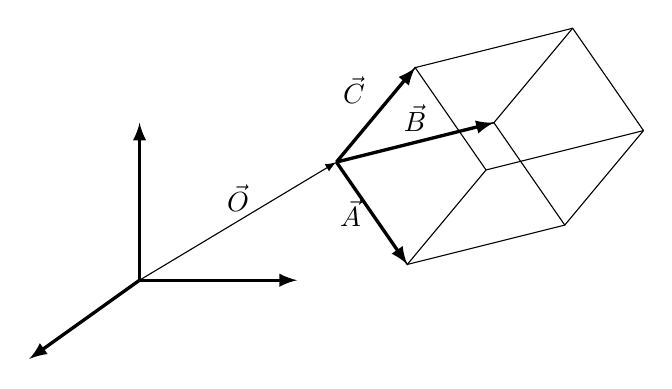
\begin{tikzpicture}[decoration={markings,mark= at position 0.5 with {\arrow{stealth}}}]
\coordinate (O) at (2.5,1.5);
\coordinate (A) at (0.9,-1.3);
\coordinate (B) at (2,0.5);
\coordinate (C) at (1,1.2);
\coordinate (C) at (1,1.2);
\draw [very thick,-latex] (0,0) -- (2,0);
\draw [very thick,-latex] (0,0) -- (0,2);
\draw [very thick,-latex] (0,0) -- (-1.4,-1);
\draw [-latex] (0,0) -- (O) node [midway,above] {$\vec O$};
\draw (O) -- ++(A) -- ++(B) -- ++(C);
\draw (O) -- ++(A) -- ++(C) -- ++(B);
\draw (O) -- ++(B) -- ++(A);
\draw (O) -- ++(B) -- ++(C);
\draw (O) -- ++(C) -- ++(A);
\draw (O) -- ++(C) -- ++(B) -- ++(A);
\draw [very thick,-latex] (O) -- ++(A) node [midway,left]{$\vec A$};
\draw [very thick,-latex] (O) -- ++(B) node [midway,above]{$\vec B$};
\draw [very thick,-latex] (O) -- ++(C) node [midway,above left]{$\vec C$};
\end{tikzpicture}\end{center}


%\subsection[add\_vect\_tri]{\lfc{add\_vect\_tri}(\lft{xO},\lft{yO},\lft{zO},\lft{xA},\lft{yA},\lft{zA},\lft{xB},\lft{yB},\lft{zB},\lft{xC},\lft{yC},\lft{zC},\lft{P},\lin{index})}
%
%\langswitch
%{
%	Définit une section triangulaire d'indice \lin{index} incluse dans un parallélépipède. L'origine de celui-ci est donnée par le vecteur $\vec O$, tandis que les trois vecteurs $\vec A$, $\vec B$ et $\vec C$ définissent ses côtés. Ces vecteurs n'ont pas à prendre en compte l'origine. Le paramètre \lft{P} détermine la position de la pointe du triangle. Pour plus de précisions, voir la figure \ref{addvtri_fig}.\\ Exemple:
%}{
%	Defines a triangular section of index \lin{index}, imbedded in a parallelepiped. Its offset is given through the $\vec O$ vector, while the $\vec A$, $\vec B$ and $\vec C$ vectors define the edges. Those three vectors do not need to take the offset into account (c.f. figure \ref{addvblock_fig}).\\ Example:
%}
%\begin{lstlisting}
%add_vect_tri(200e-9,100e-9,50e-9,
%             10e-9,15e-9,0,
%             5e-9,10e-9,0,
%             0,0,10e-9,0.5,2)
%\end{lstlisting}
%
%\begin{figure}[!ht]
%\center\def\svgwidth{0.5\linewidth}
%{\import{fig/}{vect_tri.pdf_tex}}
%\langswitch
%{
%	\caption{Schéma du volume défini par la fonction \lfc{add\_vect\_tri}.}
%}{
%	\caption{Region defined through the \lfc{add\_vect\_tri} function.}
%}
%\label{addvtri_fig}
%\end{figure}

\subsection{Non shape functions}

\subsubsection[default\_material]{\lfc{default\_material}(\lin{index})}

Fills the whole grid with the index \lin{index}. This is mostly usefull to initialize the grid.\\ Example:
\begin{lstlisting}
set_full(0)
\end{lstlisting}

\subsubsection[flip]{\lfc{flip}(\lin{x},\lin{y},\lin{z})}

\subsubsection[loop]{\lfc{loop}(\lin{x},\lin{y},\lin{z})}

\subsection{Lua defined functions}

%	En plus des formes définies par les fonctions présentées précédemment, il est possible de définir de nouvelles formes par l'intermédiaire du Lua. Pour ce faire, l'utilisateur doit créer une fonction Lua respectant certaines contraintes:
%	\begin{itemize}
%		\item la fonction doit définir pour tout point de l'espace si un point est à l'intérieur ou à l'extérieur de la forme que l'utilisateur souhaite créer. Si le point est à l'intérieur, la fonction doit avoir comme résultat 1, et 0 dans le cas contraire.
%		\item le nombre d'arguments de la fonction n'est pas limité, mais les trois premières variables doivent toujours représenter $x$, $y$ et $z$.
%		\item la fonction ne doit pas tenter de s'appuyer sur des variables globales
%	\end{itemize}

Additionally to the preview basic shapes, users can define new shapes through Lua functions. To do this, the function definition shall follow a particular template.
	\fwarn

\addtocontents{toc}{\protect\setcounter{tocdepth}{2}}

\subsubsection[add\_lua\_def]{\lfc{add\_lua\_def}(\lsg{name},\lft{var\_arg...},\lin{index})}

%	Une fois la nouvelle fonction définie, il est possible de l'appeler grâce à \lfc{add\_lua\_def}. Son premier argument \lsg{name} est le nom de la fonction définie par l'utilisateur. Ensuite viennent tous les arguments de la fonction en excluant ceux référant à $x$, $y$ et $z$. Enfin, l'indice du matériau à affecter est donné par \lin{index}.

\fwarn

\subsubsection{Example}

The following example illustrates the case of a torus defined through Lua, as this shape is not one of the basic shapes.
\begin{lstlisting}
function torus(x,y,z,x0,y0,z0)
	r0=350e-9;
	a=40e-9
	b=20e-9
	
	r=math.abs(math.sqrt((x-x0)*(x-x0)+(y-y0)*(y-y0))-r0)
	h=math.abs(z-z0)
	
	rat=b*b*(1-r*r/a/a)
	
	if h*h<=rat
		then
			return 1
	end
	
	return 0;
end

add_lua_def("torus",50e-9,100e-9,50e-9,2)
\end{lstlisting}

\subsection{Meshes}

\section{Full scripts example}

\subsection{Geometry}

The following script is a full geometry script example that defines a nanorods grid.

\begin{lstlisting}
lx=300e-9
ly=300e-9
lz=150e-9

default_material(0)
add_layer("Z",0,50e-9,1)
add_block(105e-9,235e-9,0,35e-9,50e-9,70e-9,2)
add_block(0,35e-9,105e-9,235e-9,50e-9,70e-9,2)
\end{lstlisting}

First, \lft{lx}, \lft{ly} and \lft{lz} are defined. Then the whole grid is intialized with the index 0 through the \lfc{set\_full} function. A layer of index 1 is added at the bottom of the FDTD grid along the \lsg{Z} direction through \lfc{add\_layer}, and will be the substrate in the simulation. Finally, two nanorods of index 2 are defined with the function \lfc{add\_block}, and will later in the main script be associated to the gold material.

\subsection{Main script}

The following lines will instance a \lud{structure object} based on the previous script, and pass it to the FDTD solver within the main script.
\begin{lstlisting}
struct=Structure("../structures/nanorods_grid.lua")

fdtd=MODE("fdtd_normal")
...
fdtd:structure(struct)
...
\end{lstlisting}

\chapter{FDTD: scripting interface}

\label{chapter_fdtd}

\section{Common functions}

Some functions are common to some FDTD modes of the software, and are listed here.
\addtocontents{toc}{\protect\setcounter{tocdepth}{1}}

\subsection[auto\_tsteps]{\lfc{auto\_tsteps}(\lin{Nt\_max},\lin{Nt\_check},\lft{lambda\_min},\lft{lambda\_max},\lft{coeff},\lin{Np},\lsg{layout})}

This functions attemps to evaluate the advancement of a computation, and end if when results are unlikely to change much. To do so, it performs a check every \lin{Nt\_check} iterations in the following manner. 

First \lin{Np} points are randomly selected at the start of the simulation on the boundaries of the grid. Boundaries can be enabled or disabled through the \lsg{layout} argument which is a string of three characters, each of which being either \lsgnq{n}, \lsgnq{u}, \lsgnq{d} or \lsgnq{b}, which stand for \lsgnq{none}, \lsgnq{up}, \lsgnq{down} and \lsgnq{both}, in the $x$, $y$ and $z$ order. For instance \lsg{dnb} would enable the $x_\textrm{min}$, $z_\textrm{min}$ and $z_\textrm{max}$ boundaries, while \lsg{nun} would only enable the $y_\textrm{max}$ boundary.

Once the points are chosen, they are assigned a wavelength chosen between \lft{lambda\_min} and \lft{lambda\_max}, and the related fourier transforms are performed at those locations.

Then, the algorithm evaluates the convergence of those fourier transforms through iterations, by comparing the variation to amplitude ratio of each transform to the \lft{coeff} argument (typically around $10^{-4}$ or $10^{-5}$). If the ratio for a point is less than said \lft{coeff}, then the fourier transform at that point is assumed stable. Once that criterion is checked for every point, the simulation stops.

If this criterion is never met, the simulation will only end after \lin{Nt\_max} iterations.
\begin{lstlisting}
fdtd:auto_tsteps(100000,500,400e-9,1000e-9,1e-5,200,"nnb")
\end{lstlisting}

\subsection[compute]{\lfc{compute}()}

Runs the FDTD simulation at the current state, that is with all the parameters set so far. Any following changes to the parameters will be ignored.
\begin{lstlisting}
fdtd:compute()
\end{lstlisting}


\subsection[Dx]{\lfc{Dx}(\lft{dx})}

Sets the $x$ discretization to \lft{dx}.
\begin{lstlisting}
fdtd:Dx(5e-9)
\end{lstlisting}

\subsection[Dy]{\lfc{Dy}(\lft{dy})}

Sets the $y$ discretization to \lft{dy}.
\begin{lstlisting}
fdtd:Dy(5e-9)
\end{lstlisting}

\subsection[Dz]{\lfc{Dz}(\lft{dz})}

Sets the $z$ discretization to \lft{dz}.
\begin{lstlisting}
fdtd:Dz(5e-9)
\end{lstlisting}

\subsection[Dxyz]{\lfc{Dxyz}(\lft{d})}

Sets the discretization along $x$, $y$ and $z$ to \lft{d}.
\begin{lstlisting}
fdtd:Dxyz(5e-9)
\end{lstlisting}

\subsection[N\_tsteps]{\lfc{N\_tsteps}(\lin{Nt})}

Defines the number of time steps \lin{Nt} of a simulation.\\ Example
\begin{lstlisting}
fdtd:set_N_tsteps(30000)
\end{lstlisting}

\subsection[material]{\lfc{material}(\lin{index},\lsg{material\_file})}

\label{fdtd_fc_material}
Links the material file \lsg{material\_file} to the index \lin{index} defined in the simulation geometry file.\\
	Example:
\begin{lstlisting}
fdtd:material(1,"mat_lib/Glass150.lua")
\end{lstlisting}

If the related material is supposed to be of constant real refractive index, \lsg{material\_file} may be replaced with a call to \lfc{const\_material}, of which the only argument is that refractive index. A material script will be generated on the fly.\\
	Example:
\begin{lstlisting}
fdtd:material(1,const_material(1.5))
\end{lstlisting}

%\subsubsection[padding]{\lfc{padding}(\lin{x1},\lin{x2},\lin{y1},\lin{y2},\lin{z1},\lin{z2})}
%
%\langswitch
%{
%}{
%}

\subsection[padding]{\lfc{padding}(\lin{xm},\lin{xp},\lin{ym},\lin{yp},\lin{zm},\lin{zp})}

\fwarn
\begin{itemize}
	\item \lin{xm}: PML padding along $-\vec x$
	\item \lin{xp}: PML padding along $\vec x$
	\item \lin{ym}: PML padding along $-\vec y$
	\item \lin{yp}: PML padding along $\vec y$
	\item \lin{zm}: PML padding along $-\vec z$
	\item \lin{zp}: PML padding along $-\vec z$
\end{itemize}

\subsection[pml\_X]{\lfc{pml\_X}(\lin{Npml},\lft{kappa},\lft{sigma},\lft{alpha})}

Functions of the \lfc{pml\_X} kind are used to define the PMLs (absorbing boundary conditions) of a computation. There are six of them:
\begin{itemize}
	\item \lfc{pml\_xm}: PML along $-\vec x$
	\item \lfc{pml\_xp}: PML along $\vec x$
	\item \lfc{pml\_ym}: PML along $-\vec y$
	\item \lfc{pml\_yp}: PML along $\vec y$
	\item \lfc{pml\_zm}: PML along $-\vec z$
	\item \lfc{pml\_zp}: PML along $\vec z$
\end{itemize}
They take four arguments:
\begin{itemize}
	\item \lin{Npml} define the number of PML cells, usually around a dozen
	\item \lft{kappa} defines what would roughly be $\varepsilon_r$ at the PML end, and thus how it slows down waves propagating into it. A value between 15 and 25 is usually suitable.
	\item \lft{sigma} corresponds to PMLs absorption. A value of $1/\sqrt{n}$ seems usually efficient.
	\item \lft{alpha} is a shift in the complex plane of the PML spatial coordinates. It is mostly useful if PMLs encounter evanescent waves. Typically around $0.2$.
\end{itemize}
The \lft{kappa}, \lft{sigma} and \lft{alpha} coefficients are not constant along the PML axis. The first two grow together with the PML depth, while the latter decreases in value.
Example:

\begin{lstlisting}
fdtd:pml_zp(25,25,0.7,0.2)
fdtd:pml_zm(25,25,1,0.2);
\end{lstlisting}

\subsection[prefix]{\lfc{prefix}(\lsg{name})}

Names the simulation with the prefix \lsg{name}, which will be used in the name of several files written as computation results.

\subsection[polarization]{\lfc{polarization}(\lsg{pol})}

Defines the polarization of the incident field in a simulation. \lsg{pol} can be only one of those two cases: \lsg{TE} or \lsg{TM}.\\ Example:
\begin{lstlisting}
fdtd:polarization("TE")
\end{lstlisting}

\subsection[register\_sensor]{\lfc{register\_sensor}(\lud{sensor})}

Links a sensor, created through the \lfc{create\_sensor} function (c.f. section \ref{create_sensor_def}), to the simulation. \\ Example:
\begin{lstlisting}
fdtd:register_sensor(fieldmap_1550)
\end{lstlisting}

\subsection[spectrum]{\lfc{spectrum}(\lft{lambda min} , \lft{lambda max} , \lin{Nl})}

Defines the spectral range of analysis between \lft{lambda min} and \lft{lambda max} (in meters), with \lin{Nl} points homogeneously distributed between those two wavelengths. Warning: requesting too many points can increase the computation time.\\ Example:
\begin{lstlisting}
fdtd:spectrum(3000,1e-6,3e-6)
\end{lstlisting}

\subsection[structure]{\lfc{structure}(\lud{structure object})}

Links the simulation to the geometry file \lsg{geometry\_file}. For further details, see \ref{geomsection}.\\ Example:
\begin{lstlisting}
structure_obj=Structure("structures/nanorods_grid.lua")

fdtd:structure(structure_obj)
\end{lstlisting}

\subsection[struct\_append]{\lfc{struct\_append}(\lsg{lua})}

%	Cette fonction permet d'ajouter des commandes Lua à la structure spécifiée pour la simulation. La chaîne de caractères \lsg{lua} doit donc contenir un morceau de code Lua valide. Celui-ci est alors placé en fin du script de géométrie.
	\fwarn
\begin{lstlisting}
fdtd:struct_append("subdivision_modifier(2,2,2)")
\end{lstlisting}


\subsection[struct\_parameters]{\lfc{struct\_parameters}(\lsg{lua})}

%	Comme précédemment, cette fonction permet de rajouter des éléments à un fichier de géométrie. Par contre, ceux-ci seront placés en début de script. Ceci permet d'écrire des fichiers de géométrie qui s'adapteront suivant la simulation, 
\fwarn
\begin{lstlisting}
fdtd:struct_parameters("period=1")
\end{lstlisting}


\subsection[time\_mod]{\lfc{time\_mod}(\lft{fact})}

Multiplies the natural time step $\Delta t=\frac{\min(\Delta x,\Delta y,\Delta z)}{c\sqrt{3}}$ by a factor \lft{fact} that must be set between 0 and 1.

\section{Standard mode FDTD}
\addtocontents{toc}{\protect\setcounter{tocdepth}{2}}

%	Ce mode est le mode de simulation FDTD le plus élémentaire. Il ne définit aucune source par défaut et ne fait aucune analyse. Ces deux opérations doivent donc être entièrement spécifiées par l'utilisateur. Par conséquent,  La simulation est périodique ou non suivant la spécifications de PMLs.
\fwarn
\begin{lstlisting}
fdtd=MODE("fdtd")
\end{lstlisting}

\subsection{Specific functions}

The \lfc{polarization} and \lfc{spectrum} functions are disabled in this mode.

\subsubsection[register\_source]{\lfc{register\_source}(\lud{source})}

Links a source, created through the \lfc{create\_source} function (c.f. section \ref{create_source_def}), to the simulation. \\ Example:

\begin{lstlisting}
fdtd:register_source(oscillator)
\end{lstlisting}

\section{Normal incidence FDTD}

In this mode, the structure is an infinitely periodic array in the $\vec x$ and $\vec y$ directions. The incident field is a gaussian pulse propagating along $-\vec z$, for which the spectrum, and thus the analysis spectrum, is defined through the \lfc{spectrum} function. At the end of the computation several files are written onto the hard drive, each prefixed with the name given to the \lfc{prefix} function.
	
	The \lsgnq{prefix\_show\_norm.m} file can be called by MatLab or GNU Octave. It reads \lsgnq{prefix\_spectdata\_norm} and plots the reflection and transmission coefficients of the structure, with no regard for the polarization, and then the transmittivity, reflectivity and absorption.
	
	Finally, \lsgnq{prefix\_show\_norm2.m} reads the \lsgnq{prefix\_spectdata\_norm2} file and outputs a detailled plot of all the complex reflection and transmission coefficients for the three components of the electric field. The goal is to show any potential polarization rotation effect.

\subsection{Specific functions}

%\fwarn
%\subsubsection[enable\_poynting\_sensors]{\lfc{enable\_poynting\_sensor}()}
%
%\langswitch
%{
%	\textbf{\textcolor{red}{Attention: cette option demande un espace disque extrêmement important! La quantité totale d'espace disque nécessaire est approximativement de $96N_xN_yN_t$ octets. Il est impératif d'être sûr que la quantité d'espace disque disponible est suffisante avant de lancer une simulation avec cette option.}}
%}{
%	\textbf{\textcolor{red}{Warning: after enabling this option huge files will be written on the hard drive! The total size of those files will roughly be $96N_xN_yN_t$ bytes. It is extremely important that one checks there is enough free disk space before starting a simulation with this feature enabled.}}
%}

\subsubsection{PMLs}

In this mode, only the \lfc{pml\_zm} and \lfc{pml\_zp} functions are available. The other four similar functions will be disregarded if they happen to be called.

\subsection{Full script example}

\begin{lstlisting}
structure=Structure("nanorods_grid.lua")

fdtd=MODE("fdtd_normal")
fdtd:prefix("fdtd_")
fdtd:polarization("TE")
fdtd:spectrum(1e-06,2e-06,481)
fdtd:N_tsteps(20000)
fdtd:structure(structure)
fdtd:Dxyz(5e-09)
fdtd:pml_zm(25,25,1,0.2)
fdtd:pml_zp(25,25,1,0.2)
fdtd:material(0,const_material(1))
fdtd:material(1,const_material(1.5))
fdtd:material(2,"mat_lib/Au_1m_5m_Vial.lua")

fdtd:compute()
\end{lstlisting}

\section{Oblique incidence FDTD using the Aminian and Rahmat-Samii method} 

%	Comme pour l'incidence normale, ce mode considère que les structures sont périodiques suivant $\vec x$ et $\vec y$, et que le champ se propage suivant $-\vec z$. Le champ oblique est calculé par la méthode d'Aminian et Rahmat-Samii\cite{Aminian:06}, elle-même basée sur des conditions de Bloch. Une conséquence de ceci est que la méthode ne permet pas de calculer tout un spectre pour un angle donné, mais calcule tout le champ d'une simulation pour un $k_x$ particuliers. Ainsi, on a une contrainte forte pour chaque simulation:
%	\begin{equation}
%		\lambda\sin\vartheta=\textrm{Constante}
%	\end{equation}
%	ce qui implique l'angle d'incidence varie en fonction de la longueur d'onde.

	\fwarn
	\cite{Aminian:06}
	\begin{equation}
		\lambda\sin\vartheta=\textrm{Constant}
	\end{equation}

\subsection{Specific functions}

\subsubsection[kx\_auto]{kx\_auto(\lft{ang\_min},\lft{ang\_max})}

\subsubsection[kx\_fixed\_angle]{kx\_fixed\_angle(\lin{Nkx},\lft{lambda\_min},\lft{lambda\_max},\lft{angle})}

Runs \lin{Nkx} simulations for a specific angle \lft{angle}, with the target wavelength varying between \lft{lambda\_min} and \lft{lambda\_max}.

\subsubsection[kx\_fixed\_lambda]{kx\_fixed\_lambda(\lin{Nkx},\lft{lambda},\lft{ang\_min},\lft{ang\_max})}

\fwarn

\subsubsection[kx\_target]{kx\_target(\lft{lambda},\lft{angle})}

%	Effectue une simulation en visant un angle particulier \lft{angle} pour une longueur d'onde donnée \lft{lambda}.
	\fwarn

\subsubsection{PMLs}

In this mode, only the \lfc{pml\_zm} and \lfc{pml\_zp} functions are available. The other four similar functions will be disregarded if they happen to be called.

\subsection{Real script example}

\begin{lstlisting}
structure=Structure("structures_priv/hexa_cones_s150_h300_inv.lua")

fobl=MODE("fdtd_oblique_ARS")
fobl:prefix("fobl_");
fobl:polarization("TE");
fobl:kx_fixed_lambda(3,425e-9,10,60)
fobl:structure(structure);
fobl:N_tsteps(100000);
fobl:spectrum(3000,400e-9,450e-9);
fobl:pml_zp(25,25,0.7,0.2)
fobl:pml_zm(25,25,1,0.2);
fobl:material(0,"mat_lib/Ind181.lua")
fobl:material(1,"mat_lib/Fspace.lua")

fobl:compute()
\end{lstlisting}

\section{Single particles}

This is a specific mode dedicated to simulating single particles. It is called through
\begin{lstlisting}
fdtd=MODE("fdtd_single_particle")
\end{lstlisting}
In this mode, the user can choose the periodicity of the structure. For instance, if the \lfc{pml\_x} functions are not used the software will consider the structure is periodic along $x$. No analysis is performed, and that so this part is left to the user.


\subsection{Specific functions}


\subsubsection[structure\_aux]{\lfc{structure\_aux}(\lsg{geometry\_file})}

This function is used to specify an auxiliary structure for the simulation. This structure is used for the padding around the main geometry, and is used to compute the incident field. If the function is not used the software will just use the main grid at $x=0$, $y=$ as the auxiliary grid.

\subsection{Real script example}

\begin{lstlisting}
structure=Structure("structures/donut_cavity_aux.lua")

fdonut=MODE("fdtd_single_particle")
fdonut:prefix(prefix);
fdonut:polarization("TE");
fdonut:structure(structure);
fdonut:structure_aux();
fdonut:auto_tsteps(100000,500,400e-9,1000e-9,1e-5,200);
fdonut:spectrum(3001,400e-9,1000e-9);
fdonut:pml_xp(25,25,1,0.2);
fdonut:pml_xm(25,25,1,0.2);
fdonut:pml_yp(25,25,1,0.2);
fdonut:pml_ym(25,25,1,0.2);
fdonut:pml_zp(25,25,1,0.2);
fdonut:pml_zm(25,25,0.8,0.2);
fdonut:material(0,"mat_lib/Fspace.lua")
fdonut:material(1,"mat_lib/Glass150.lua")
fdonut:material(2,const_material(index))
fdonut:material(3,"mat_lib/V_Au_400_1000_PCRC2.lua")

fdonut:compute()
\end{lstlisting}


\section{Sensors}

\label{create_sensor_def}

\subsection{Common functions}

\subsubsection[location]{\lfc{location}(\lin{x1},\lin{x2},\lin{y1},\lin{y2},\lin{z1},\lin{z2})}

Sets the sensor location between \lin{x1}, \lin{y1}, \lin{z1} (inclus) and \lin{x2}, \lin{y2}, \lin{z2} (exclus). Those coordinates must be defined with respect to the computation geometry file, and this can be negative.

\subsubsection[name]{\lfc{name}(\lsg{name})}

Gives the sensor the name \lsg{name}, which will serve as a prefix to the names of the files written at the end of the computation.

\subsubsection[orientation]{\lfc{orientation}(\lsg{orientation})}

This defines the sensor orientation (its normal vector), through the \lsg{orientation} variable. Its value can be \lsg{X}, \lsg{Y}, \lsg{Z}, \lsg{-X}, \lsg{-Y} or \lsg{-Z}. This function has two main goals:
\begin{itemize}
	\item setting a direction onto which the Poynting vector will be projected, for the sensors that need it.
	\item specifying the exact location of the sensor, which was previously defined through the \lfc{location} function. For instance, if the orientation is \lsg{X} or \lsg{-X} the \lin{x2} variable will be ignored. Similarly, \lsg{Y} will affect \lin{y2} and \lsg{Z} will affect \lin{z2}.
\end{itemize}

\subsubsection[spectrum (one argument)]{\lfc{spectrum}(\lft{lambda})}

Sets the sensor analysis wavelength \lft{lambda}.

\subsubsection[spectrum (three arguments)]{\lfc{spectrum}(\lft{lambda\_min},\lft{lambda\_max},\lin{Nl})}

Sets the sensor analysis spectrum between \lft{lambda\_min} and \lft{lambda\_max}, with \lin{Nl} sampling points.

\subsection{Sensor types}

\subsubsection{fieldmap}

This sensors is dedicated to creating 2D fieldmaps. The fieldmap is computed for a single wavelength, specified through the single argument variant of \lfc{spectrum}.
	
At the end of the simulation, several files are created:
\begin{itemize}
	\item \lsgnq{name\_fieldmap.bmp}: a quick fieldmap image using a non-linear normalization
	\item \lsgnq{name.m}: a MatLab script that will display the fieldmap
	\item \lsgnq{name\_Ex\_raw}: a file containing the sensor data for the $x$ component of the field
	\item \lsgnq{name\_Ey\_raw}: a file containing the sensor data for the $x$ component of the field
	\item \lsgnq{name\_Ez\_raw}: a file containing the sensor data for the $x$ component of the field
\end{itemize}
Example:
\begin{lstlisting}
map=create_sensor("fieldmap")
map:spectrum(405e-9)
map:name("map")
map:orientation("Y")
map:location(0,500,0,1,0,500)

fdtd:register_sensor(map)
\end{lstlisting}

\subsubsection{fieldblock}

\subsubsection{planar\_spectral\_poynting}

\fwarn
This sensor integrates the Poynting vector flux across a planar surface.


\section{Light sources}

\label{create_source_def}

\subsection{Common functions}

\subsubsection[location (three arguments)]{\lfc{location}(\lin{x1},\lin{y1},\lin{z1})}

Set the source location at (\lin{x1}, \lin{y1}, \lin{z1}). Those coordinates must be defined with respect to the computation geometry file, and this can be negative.

\subsubsection[location (six arguments)]{\lfc{location}(\lin{x1},\lin{x2},\lin{y1},\lin{y2},\lin{z1},\lin{z2})}

Set the source location between \lin{x1}, \lin{y1}, \lin{z1} (included) and \lin{x2}, \lin{y2}, \lin{z2} (excluded). Those coordinates must be defined with respect to the computation geometry file, and this can be negative.

\subsubsection[orientation]{\lfc{orientation}(\lsg{orientation})}

Defines the source orientation, that is \lsg{X}, \lsg{Y} or \lsg{Z}. This function is only ûsed by point sources.

\subsubsection[spectrum (one argument)]{\lfc{spectrum}(\lft{lambda})}

Defines the source wavelength as \lft{lambda}.

\subsubsection[spectrum (two arguments)]{\lfc{spectrum}(\lft{lambda\_min},\lft{lambda\_max})}

Defines the source spectrum as gaussian, between \lft{lambda\_min} and \lft{lambda\_max}.

\subsection{Source types}

\subsubsection{oscillator}

This source adds field to the simulation grid at each time step. This done through a operation like:

\begin{equation}
	E(t+1)=E(t)+sin(\omega t)
\end{equation}

As such, this souce is not exactly a radiating electric dipole, but just shows a similar behavior. Furthermore, field injection method can potentially create a static electric and magnetic field at the end of the simulation, and so this source must be used with care.
	
	This is a point source, and so its location is specified through the three arguments variant of the \lfc{location} function. The excited field component is set by the \lfc{orientation} function. The source has a wide spectrum, and so the two arguments variant of the \lfc{spectrum} function needs to be used.\\ Example:

\begin{lstlisting}
src=create_source("oscillator")
src:location(250,0,410)
src:orientation("Z")
src:spectrum(300e-9,1000e-9)

fdtd:register_source(src)
\end{lstlisting}

\subsubsection{Electric dipole}

Todo.

\subsubsection{Magnetic dipole}

Todo.
	

\chapter{FDTD: GUI}

%%%%%%%%%%%%%%%%%
%   Ray Optics
%%%%%%%%%%%%%%%%%

\part{Ray optics: Selene}

\chapter{Selene: scripting interface}

\section{Principles}

\subsection{Organization}

Raytracing calculations are done by setting a scene up and feeding it to a renderer. This is first done by calling \lfc{MODE}(\lsg{selene}) which returns an instance of the Selene renderer. It only has a few functions that can modify it.

The first one is \lfc{N\_rays\_total}(\lin{N}) which will set the total number of rays that need to be computed.

Then the user has to define the optical elements, light sources, materials, etc, and feed them to the rendered. This is done by \lfc{add\_object}(\lud{object}) where \lud{object} is a Selene object, and \lfc{add\_light}(\lud{light}) where \lud{light} is a Selene light source.

Once this is done, the user needs to call \lfc{render}() to start the computation. This function can be called several times to run several simulations in a raw, after modifying an object's properties for instance.

Eventually, a typical script will look like
\begin{lstlisting}
sln=MODE("selene")
sln:N_rays_total(2000000)

% Scene definition

sln:add_object(object_1)
sln:add_object(object_2)
sln:add_light(source)

sln:render()
\end{lstlisting}

\subsection{Inner workings}

This is a summary of the rendering algorithm:

\begin{enumerate}
	\item At the beginning of the rendering the object and light sources locations are recomputed based on other objects. Various other properties can be computed, or memory or files allocated.
	\item A ray is created from one of the registered light sources and is fetched by renderer
	\item The intersection between this ray and every object is computed
		\begin{itemize}
			\item First, by computing the intersection with the bounding box first to have a quick approximation
			\item Then by computing the intersection with the various faces of the object, if the first step showed potential intersection
		\end{itemize}
	\item The intersections are looked through for the one with the smallest positive time, and the others are discarded
	\item The object related to that intersection is asked to treat the ray based on the face intersected and the intersection location
	\item It is determined from which side of the face (up or down, see \ref{faces_irfs}) the ray is coming
	\item The relevant Interface Response Function is given the ray and the refractive index of each side of the face, and determines how the ray must be redirected based or absorbed based on its optical properties
	\item Intersections for the new ray are computed again until it is either absorbed or lost
	\item The renderer fetches a new ray until the required number of rays has been computed
\end{enumerate}

\subsection{Probabilistic behavior}

\label{selene_probabilistic}
Raytracing usually follows a Monte-Carlo approach, that is to say one generates many random rays in a scene, and cast them with random directions and/or locations based on the properties of the sources, and have them intersect with objects.

How you handle those interactions, however, can be of two kinds: patch branching and probabilistic. To illustrate path branching, let's assume one computes the interaction of a ray with a glass surface. The transmission and reflection coefficients are not zero, so from one incident ray two would be generated. Those would then propagate again and generate new rays and so on. One can immediately notice that, in pathological cases, this could make the number of rays grow exponentially. Given enough computational time, it should be possible to address all of them, but then a lot of CPU time would have been spent computing the children of only one initial ray, giving much weight to that particular location.

With Selene, we have chosen to go with a full probabilistic approach. If an interface has a reflection, transmission, and absorption coefficient, energy conservation requires that
\begin{equation}
	R+T+A=1
\end{equation}
If one interprets this probabilistically, that means the sum of the probabilities for the ray to be reflected, transmitted or absorbed is 1. Another way to see it, is that one could split the numbers between 0 and 1 into three regions of lengths $R$, $T$ and $A$ as follows:
\begin{center}\begin{tikzpicture}
\draw [thick] (0,0) -- (10,0);
\draw [thick] (0,-0.5) -- (0,0.5);
\draw [thick] (10,-0.5) -- (10,0.5);
\draw [thick] (3,-0.5) -- (3,0.5);
\draw [thick] (8,-0.5) -- (8,0.5);
\draw (1.5,0) node[above]{$R$};
\draw (5.5,0) node[above]{$T$};
\draw (9,0) node[above]{$A$};
\draw (0,0.5) node[above]{0};
\draw (10,0.5) node[above]{1};
\draw [thick,-latex] (0,-1) -- (6,-1);
\draw (6,-1) node[right]{$p$};
\end{tikzpicture}\end{center}
if one takes a random number $p$ between 0 and 1, the region p falls in will determine the result of the calculation. This approach can be generalized to any number of effects the resulting ray could encounter. This ensures that one ray can only give rise to at most one ray.

While the probabilistic approach does not compute the exact behavior of a specific point, it will still statistically properly reconstruct the behavior of the whole neighborhood of it.

\subsection{Simulation summary}

After each call of \lfc{render} the program outputs a summary log under the file name \lsgnq{selene\_render\_X} within the \lfc{output\_directory}, where \lsgnq{X} is the render number, starting from 0. This file is a mini-script that specifies
\begin{itemize}
	\item the requested number of rays
	\item the power of each source
	\item the number of ray of each source
	\item the power carried by each ray
\end{itemize}

Its purpose is for the analysis of results after the render, for some of this information will be required.

\section{Relative positioning}

Selene's positioning system can be relative. That means objects can be placed relatively to others, or the world's origin of course.

\subsection{Orientation}

\label{selene_relative_positioning}
The first part of the positioning system is defining the object's orientation. Each object comes with its own frame, and most object primitives are aligned with a particular axis within this frame. For instance, the axis of a cylinder is aligned with the $\vec x$ axis of the object's frame. To rotate the cylinder in the world, one thus needs to rotate the frame itself.

This rotation is specified through Euler angles. The convention chosen in this software is yaw$\rightarrow$pitch$\rightarrow$roll, or $zy'x"$. That is, first the frame is rotated by an angle $\alpha$ around $\vec z$, then by an angle $\beta$ around the new $\vec y$ axis, and finally by an angle $\gamma$ around the new $\vec x$ axis.

\begin{center}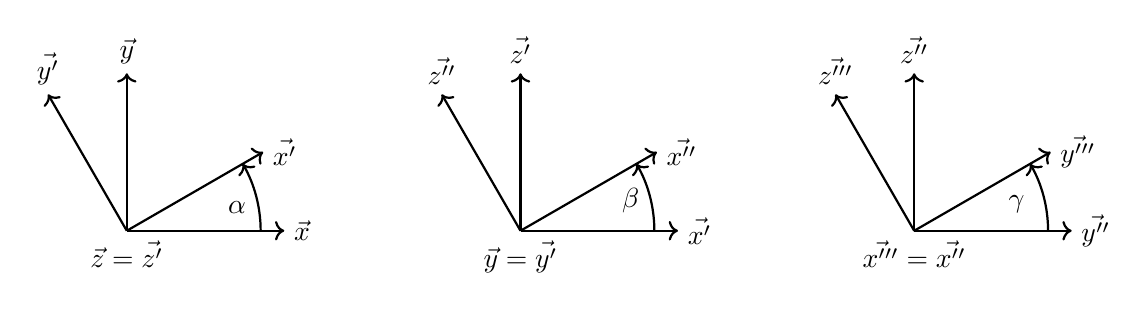
\begin{tikzpicture}
\draw [thick,->] (0,0) -- (2,0);
\draw [thick,->] (0,0) -- (0,2);
\draw (2,0) node[right]{$\vec{x}$};
\draw (0,2) node[above]{$\vec{y}$};
\draw (0,0) node[below]{$\vec{z}=\vec{z'}$};
\draw [thick,->](1.7,0) arc [start angle=0, end angle=30, radius=1.7];
\draw [thick,->] (0,0) -- (1.7321,1);
\draw [thick,->] (0,0) -- (-1,1.7321);
\draw (1.7321,1) node[right]{$\vec{x'}$};
\draw (-1,1.7321) node[above]{$\vec{y'}$};
\draw (1.4,0.1) node[above]{$\alpha$};

\draw [thick,->] (5,0) -- (7,0);
\draw [thick,->] (5,0) -- (5,2);
\draw (7,0) node[right]{$\vec{x'}$};
\draw (5,2) node[above]{$\vec{z'}$};
\draw (5,0) node[below]{$\vec{y}=\vec{y'}$};
\draw [thick,->](6.7,0) arc [start angle=0, end angle=30, radius=1.7];
\draw [thick,->] (5,0) -- (6.7321,1);
\draw [thick,->] (5,0) -- (4,1.7321);
\draw (6.7321,1) node[right]{$\vec{x''}$};
\draw (4,1.7321) node[above]{$\vec{z''}$};
\draw (6.4,0.1) node[above]{$\beta$};

\draw [thick,->] (10,0) -- (12,0);
\draw [thick,->] (10,0) -- (10,2);
\draw (12,0) node[right]{$\vec{y''}$};
\draw (10,2) node[above]{$\vec{z''}$};
\draw (10,0) node[below]{$\vec{x'''}=\vec{x''}$};
\draw [thick,->](11.7,0) arc [start angle=0, end angle=30, radius=1.7];
\draw [thick,->] (10,0) -- (11.7321,1);
\draw [thick,->] (10,0) -- (9,1.7321);
\draw (11.7321,1) node[right]{$\vec{y'''}$};
\draw (9,1.7321) node[above]{$\vec{z'''}$};
\draw (11.3,0.1) node[above]{$\gamma$};
\end{tikzpicture}\end{center}

 Now, this rotation can either be absolute, or relative to another object. In the latter case, the reference rotation frame will need to be set through the \lfc{rotation\_frame}(\lud{object}) function. The frame of the object we want to manipulate will be set identical to the frame of the reference, and then rotated.

\subsection{Placement}

The second part of the system is relative locations. Once an objet's orientation is set, it can be placed in the scene relatively to the world's origin or to another object. The purpose is to define object groups that can move with eachother. Now, this relative location does not necessarily need to be defined from an object's origin to another's. Indeed, some objects have particular points of interest, and it can be useful to place objects relatively to those points. For instance, two lenses can be aligned so that their focal points match. In this case, the relative locations of the lenses' centers is irrelevant. Those points will be called anchors, and each object type will have its own anchors depending on its parameters.

The process is illustrated with the figure below.
\begin{center}
\begin{tikzpicture}[scale=2.5]
\draw (0,0) node[below left]{O$_1$};
\draw [thick,->] (-0.5,0) -- (1,0);
\draw [thick,->] (0,-0.5) -- (0,1);
\draw (1,0) node[below]{$\vec{x_1}$};
\draw (0,1) node[left]{$\vec{y_1}$};
\draw (1.1,0.8) -- (1.3,0.8);
\draw (1.2,0.7) -- (1.2,0.9);
\draw (1.2,0.8) node[below]{A};
\draw [red,thick,->] (0.767,1.05) -- (2.066,0.3);
\draw [red,thick,->] (0.95,0.367) -- (1.7,1.666);
\draw (2.0666,0.3) node[red,below]{$\vec{x_D}$};
\draw (1.7,1.666) node[red,above left]{$\vec{y_D}$};
\draw [blue] (2.9,2) -- (3.1,2);
\draw [blue] (3,1.9) -- (3,2.1);
\draw (3,2) node[blue,above left]{B};
\draw [dgreen,thick,->] (1.2,0.8) -- (3,2);
\draw (2.1,1.4) node[dgreen,below]{$\vec{D}$};
\draw [blue,thick,->] (3.35,1.933) -- (4.1,0.634);
\draw [blue,thick,->] (3.167,1.25) -- (4.466,2);
\draw (3.6,1.5) node[blue,below]{O$_2$};
\draw (4.1,0.634) node[blue,right]{$\vec{x_2}$};
\draw (4.466,2) node[blue,right]{$\vec{y_2}$};
\end{tikzpicture}\end{center}
In this, we have two objects O$_1$ and O$_2$. First, O$_2$ had its orientation set, which is different from O$_1$'s orientation. O$_1$ has an anchor A, and O$_2$ an anchor B, and we want both anchors to be displaced relatively to eachother through the vector $\vec D$. Moreover, $\vec D$ itself can be expressed in a frame that is independent from O$_1$ and O$_2$. We will then define the following properties for O$_2$:
\begin{itemize}
	\item B will be its new origin
	\item A, belonging to O$_1$, will be set as its displacement reference.
	\item the frame D will be set based on any other frame in the scene, and $\vec D$ will be defined within it
\end{itemize}	
We will then have
\begin{equation}
	\vec{O_2}=\vec{O_1}+\vec{O_1 A} + \vec D+\vec{B O_2}
\end{equation}

\section{Faces and Interface Response Functions}

\label{faces_irfs}

\subsection{Face orientation}

\subsubsection{Up and Down}

The core elements with which rays in Selene interact are the faces of the various objects of a scene, and this section aims to describes what happens.

Faces come in favious shapes. They can be a plane, a parabola, a triangle, etc. In every case, faces have two sides, and the software is made so that do not necessarily behave the same sway. We thus need to be able to differentiate both sides, and this is done by the orientation of the normal vector to a face.

The direction towards which the normal vector is pointing will be known as ``up'', or the outside of a closed surface, and the opposite direction will be known as ``down'', or the inside of a closed surface.
\begin{figure}[!ht]
\begin{center}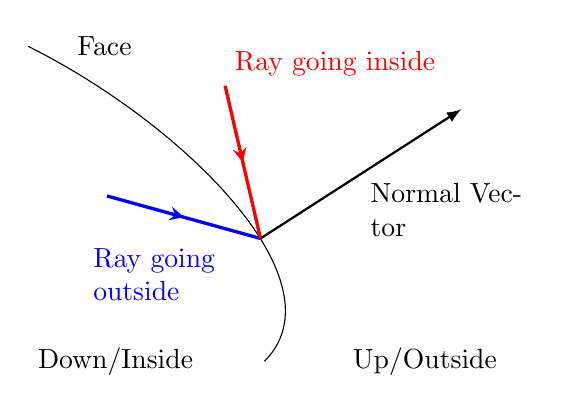
\begin{tikzpicture}[decoration={markings,mark= at position 0.5 with {\arrow{stealth}}}]
\draw (0,4) .. controls (2,3) and (4,1) .. (3,0);
\draw (0.5,4) node[right]{Face};
\draw (0,0) node[right]{Down/Inside};
\draw (4,0) node[right]{Up/Outside};
\draw [ thick,-latex] (2.95,1.56) -- (5.5,3.2);
\draw (4.225,2.38) node[below right,text width=2cm]{Normal Vector};
\draw [very thick,-,blue,postaction={decorate}] (1,2.1) -- (2.95,1.56);
\draw (2.95,1.56) node[blue,below left,text width=2cm]{Ray going outside};
\draw [very thick,-,red,postaction={decorate}] (2.5,3.5) -- (2.95,1.56);
\draw (2.5,3.5) node[red,above right]{Ray going inside};
\end{tikzpicture}\end{center}
\caption{Conventions around faces in Selene}
\end{figure}
The direction of the normal vector determines how an incident ray will interact with the face. If the scalar product between the direction vector of a ray and the normal factor of the face is positive, then the ray is going outside, and will be treated using the ``down'' properties of the face. If that scalar product is negative, the ray is going inside, and will be treated using the ``up'' properties.

\subsubsection{Properties of each side}

The most obvious property difference between the up and down sides is the material they refer to. After all, faces are supposed to represent where there is a change in refractive index. As such, each side will point to a different material defined by the user. Note that in some cases, like a transparent sensor surface that is not supposed to modify rays, the materials of both sides can be the same.

But merely knowing the materials is not enough to define what will happen to an incident ray. Indeed, while one could just use them to compute refraction and reflection, this is not the only way a surface can behave. Photons can be scattered, diffracted, absorbed, etc. To handle those different behaviors, we use what we call an Interface Response Function, or IRF. The purpose of the IRF will be to redirect a ray or destroy it depending of the various properties of the face.

We've chosen to make it so that both sides of a face don't necessarily have the same IRF. It can be used to define non-physical, but convenient, behaviors such as a face being perfectly antireflective from one side, and perfectly reflective from the other, or to input simulation data for both sides (the behavior of nanostructures for  instance will not be perfectly symmetrical). As such, both sides will refer to a potentially different IRFs.

Certains IRFs will require complete frames to determine the direction of the outgoing ray. In the case of Snell's law such a frame can be determined from the normal vector and the ray direction alone, but this would not work with a diffraction grating. As such, faces have an additional properties: a tangent vector. This vector is specified per face, per side, and can be fixed or have a special configuration that will adapt to the face. More details are to be found in the objects descriptions.

\subsection{The Interface Response Function}

As stated before, the purpose of the Interface Response Function is to turn an incident ray into a reflected or transmitted ray, or to absorb it, in the manner described in section \ref{selene_probabilistic}. This this done in accordance to the refractive index of the related face and its tangent vector.

To each specific optical behavior corresponds an IRF. See the section \ref{selene_object_funcs} to known how to assign them to objects.

\subsubsection{Default IRFs}

There are several default, basic IRFs, than can be passed to objects. They are
\begin{itemize}
	\item[] \textbf{SEL\_IRF\_FRESNEL}: the interface's response obeys the Fresnel coefficients of the associated materials, while the 
	\item[] \textbf{SEL\_IRF\_PERFECT\_ABSORBER}: all rays hitting the interface are absorbed and disappear
	\item[] \textbf{SEL\_IRF\_PERFECT\_ANTIREFLECTOR}: all rays hitting an interface go through it, but still obey Snell's law
	\item[] \textbf{SEL\_IRF\_PERFECT\_MIRROR}: rays are always reflected
\end{itemize}

\subsubsection{User defined IRFs}

\newpage
\section{Objects}

Selene objects are added through the function \lfc{Selene\_object}(\lsg{type},\lft{args}). Here, \lft{args} is actually a variable sequence of argument depending on the object \lud{type}. For instance, a sphere will only have one possible argument, its radius, while a cylinder will have two: its length and radius. This function returns an object which can then be manipulated in the script (see \ref{selene_object_funcs}).

\noindent Usage example:
\begin{lstlisting}
obj=Selene_object("cylinder",0.5,5.0)
\end{lstlisting}

\subsection{Functions common to all objects}

\label{selene_object_funcs}
%\addtocontents{toc}{\protect\setcounter{tocdepth}{2}}

\subsubsection[contains]{\lfc{contains}(\lft{x},\lft{y},\lft{z})}

Returns 1 if the object contains the point defined by $(x,y,z)$, and zero otherwise. Only valid for volume objects. It can still be called with the others but will return an undefined value.
\begin{lstlisting}
var=obj:contains(0.25,0,1.5)
\end{lstlisting}

\subsubsection[default\_in\_IRF]{\lfc{default\_in\_IRF}(\lud{IRF})}

Sets the IRF for every face of the object, on the down side, to \lud{IRF}.
\begin{lstlisting}
obj:default_in_IRF(SEL_IRF_PERFECT_ABSORBER)
\end{lstlisting}

\subsubsection[default\_in\_mat]{\lfc{default\_in\_mat}(\lud{Material})}

Sets the material for every face of the object, on the down side, to \lud{Material}.
\begin{lstlisting}
obj:default_in_mat(Glass)
\end{lstlisting}

\subsubsection[default\_IRF]{\lfc{default\_IRF}(\lud{IRF})}

Sets the IRF for every face of the object, on the both sides, to \lud{IRF}.
\begin{lstlisting}
obj:default_IRF(SEL_IRF_FRESNEL)
\end{lstlisting}

\subsubsection[default\_out\_IRF]{\lfc{default\_out\_IRF}(\lud{IRF})}

Sets the IRF for every face of the object, on the up side, to \lud{IRF}.
\begin{lstlisting}
obj:default_out_IRF(SEL_IRF_PERFECT_MIRROR)
\end{lstlisting}

\subsubsection[default\_out\_mat]{\lfc{default\_out\_mat}(\lud{Material})}

Sets the material for every face of the object, on the up side, to \lud{Material}.
\begin{lstlisting}
obj:default_out_mat(Air)
\end{lstlisting}

\subsubsection[face\_down\_IRF]{\lfc{face\_down\_IRF}(\lin{face number},\lud{IRF})}

Sets the down IRF of the face indexed by \lin{face number} (starting at 0) to \lud{IRF}.
\begin{lstlisting}
obj:face_down_IRF(0,SEL_IRF_PERFECT_ANTIREFLECTOR)
\end{lstlisting}

\subsubsection[face\_down\_mat]{\lfc{face\_down\_mat}(\lin{face number},\lud{Material})}

Sets the down material of the face indexed by \lin{face number} (starting at 0) to \lud{Material}.
\begin{lstlisting}
obj:face_down_mat(12,sapphire)
\end{lstlisting}

\subsubsection[face\_down\_tangent (two arguments)]{\lfc{face\_down\_tangent}(\lin{face number},\lsg{type})}

Sets type of the down tangent of the face indexed by \lin{face number} (starting at 0) to \lsgnq{type}. See the objects properties for more details.
\begin{lstlisting}
obj:face_down_tangent(4,"polar")
\end{lstlisting}

\subsubsection[face\_down\_tangent (four arguments)]{\lfc{face\_down\_tangent}(\lin{face number},\lft{x},\lft{y},\lft{z})}

Sets =the down tangent of the face indexed by \lin{face number} to the vector (\lft{x},\lft{y},\lft{z}).
\begin{lstlisting}
obj:face_down_tangent(0,1,0,0)
\end{lstlisting}

\subsubsection[face\_IRF]{\lfc{face\_IRF}(\lin{face number},\lud{IRF})}

Sets the IRF of the face indexed by \lin{face number} (starting at 0), on both sides, to \lud{IRF}.
\begin{lstlisting}
obj:face_IRF(0,SEL_IRF_FRESNEL)
\end{lstlisting}

\subsubsection[face\_up\_IRF]{\lfc{face\_up\_IRF}(\lin{face number},\lud{IRF})}

Sets the up IRF of the face indexed by \lin{face number} (starting at 0) to \lud{IRF}.
\begin{lstlisting}
obj:face_up_IRF(2,SEL_IRF_PERFECT_ANTIREFLECTOR)
\end{lstlisting}

\subsubsection[face\_up\_mat]{\lfc{face\_up\_mat}(\lin{face number},\lud{Material})}

Sets the up material of the face indexed by \lin{face number} (starting at 0) to \lud{Material}.
\begin{lstlisting}
obj:face_up_mat(1,Air)
\end{lstlisting}

\subsubsection[face\_up\_tangent (two arguments)]{\lfc{face\_up\_tangent}(\lin{face number},\lsg{type})}

Sets type of the up tangent of the face indexed by \lin{face number} (starting at 0) to \lsgnq{type}. See the objects properties for more details.
\begin{lstlisting}
obj:face_up_tangent(2,"polar_neg")
\end{lstlisting}

\subsubsection[face\_up\_tangent (four arguments)]{\lfc{face\_up\_tangent}(\lin{face number},\lft{x},\lft{y},\lft{z})}

Sets the up tangent of the face indexed by \lin{face number} to the vector (\lft{x},\lft{y},\lft{z}).
\begin{lstlisting}
obj:face_up_tangent(4,0,1,0)
\end{lstlisting}

\subsubsection[location]{\lfc{location}(\lft{x},\lft{y},\lft{z})}

Sets the object location to (\lft{x},\lft{y},\lft{z}) within the translation frame. The true location will be defined according to the relative positioning system. See \ref{selene_relative_positioning} for a detailled explanation.
\begin{lstlisting}
obj:location(1,1,0)
\end{lstlisting}

\subsubsection[name]{\lfc{name}(\lsg{object name})}

Sets the object name to \lsgnq{name}.
\begin{lstlisting}
obj:name("main_lens")
\end{lstlisting}

\subsubsection[origin]{\lfc{origin}(\lsgnq{anchor name})}

Sets the origin of the object to its anchor defined by \lsgnq{anchor name}. See \ref{selene_relative_positioning} for more details, and the objects descriptions for a list of the anchors.
\begin{lstlisting}
obj:origin(SEL_OBJ_BOX_FACE_XP)
\end{lstlisting}

\subsubsection[relative\_origin]{\lfc{relative\_origin}(\lud{relative frame},\lsgnq{anchor name})}

Sets the relative origin of the object to anchor of the \lud{relative frame} designed by \lsgnq{anchor name}. See \ref{selene_relative_positioning} for more details, and the objects descriptions for a list of the anchors.
\begin{lstlisting}
obj:relative_origin(object_0,SEL_OBJ_BOX_CORNER_XM_YM_ZM)
\end{lstlisting}

\subsubsection[rotation]{\lfc{rotation}(\lft{$\alpha$},\lft{$\beta$},\lft{$\gamma$})}

Set the angles of rotation of the object to \lft{$\alpha$}, \lft{$\beta$} and \lft{$\gamma$}, in degrees, relative to the \lud{rotation frame}. See \ref{selene_relative_positioning} for more details.
\begin{lstlisting}
obj:rotation(45,20,0)
\end{lstlisting}

\subsubsection[rotation\_frame]{\lfc{rotation\_frame}(\lud{frame})}

Set the relative rotation frame of the object the to one held by \lud{frame}. See \ref{selene_relative_positioning} for more details.
\begin{lstlisting}
obj:rotation_frame(object_1)
\end{lstlisting}

\subsubsection[translation\_frame]{\lfc{translation\_frame}(\lud{frame})}

Set the relative translation frame of the object to the one held by \lud{frame}. See \ref{selene_relative_positioning} for more details.
\begin{lstlisting}
obj:translation_frame(object_0)
\end{lstlisting}

\subsubsection[sensor]{\lfc{sensor}(\lsg{transp}/\lsg{abs},\lsg{options 1},\lsg{options 2},...)}

Will turn the object into a sensor. See the section \ref{selene_sensors} for a full description of the options and what they do.
\begin{lstlisting}
obj:sensor("abs","wavelength","ID","obj_intersection")
\end{lstlisting}

\newpage
\subsection{Volume primitives}

Volume objects are objects that are defined by a closed surface.

\subsubsection{Box}

As its name indicates, the \lud{box} object is just a block with parallel faces, over variable width, heights and length. As such, adding one in the script will involve \lfc{Selene\_object}(\lsg{box},\lft{lx},\lft{ly},\lft{lz}), where \lft{lx} and so on will be the length along the $x$, $y$ and $z$ axes. By default, the box' origin is its center, meaning it extends from $-lx/2$ to $+lx/2$, and so on.

\noindent Example:
\begin{lstlisting}
obj=Selene_object("box",2,3,4)
\end{lstlisting}

The default anchor is the center of the \lud{box}: SEL\_OBJ\_BOX\_CENTER

However, the following specific point serve as anchors for the \lud{box} object. Here, XM refers to the first face on the $x$ axis, and XP refers to the second face on the $x$ axis. The same goes for the $y$ and $z$ axes. There are six face anchors corresponding to the center of each face, and eight corner anchors corresponding to each vertex of the box.

\begin{tabular}{|c|c|}
\hline
Faces & Corners \\
\hline
SEL\_OBJ\_BOX\_FACE\_XM & SEL\_OBJ\_BOX\_CORNER\_XM\_YM\_ZM \\
SEL\_OBJ\_BOX\_FACE\_XP & SEL\_OBJ\_BOX\_CORNER\_XP\_YM\_ZM \\
SEL\_OBJ\_BOX\_FACE\_YM & SEL\_OBJ\_BOX\_CORNER\_XM\_YP\_ZM \\
SEL\_OBJ\_BOX\_FACE\_YP & SEL\_OBJ\_BOX\_CORNER\_XP\_YP\_ZM \\
SEL\_OBJ\_BOX\_FACE\_ZM & SEL\_OBJ\_BOX\_CORNER\_XM\_YM\_ZP \\
SEL\_OBJ\_BOX\_FACE\_ZP & SEL\_OBJ\_BOX\_CORNER\_XP\_YM\_ZP \\
& SEL\_OBJ\_BOX\_CORNER\_XM\_YP\_ZP \\
& SEL\_OBJ\_BOX\_CORNER\_XP\_YP\_ZP \\
\hline
\end{tabular}


\newpage
\subsubsection{Cone}

\begin{itemize}
	\item \textbf{SEL\_OBJ\_CONE\_CENTER}
	\item \textbf{SEL\_OBJ\_CONE\_FACE}
	\item \textbf{SEL\_OBJ\_CONE\_TIP}
\end{itemize}

\newpage
\subsubsection{Cylinder}

\begin{center}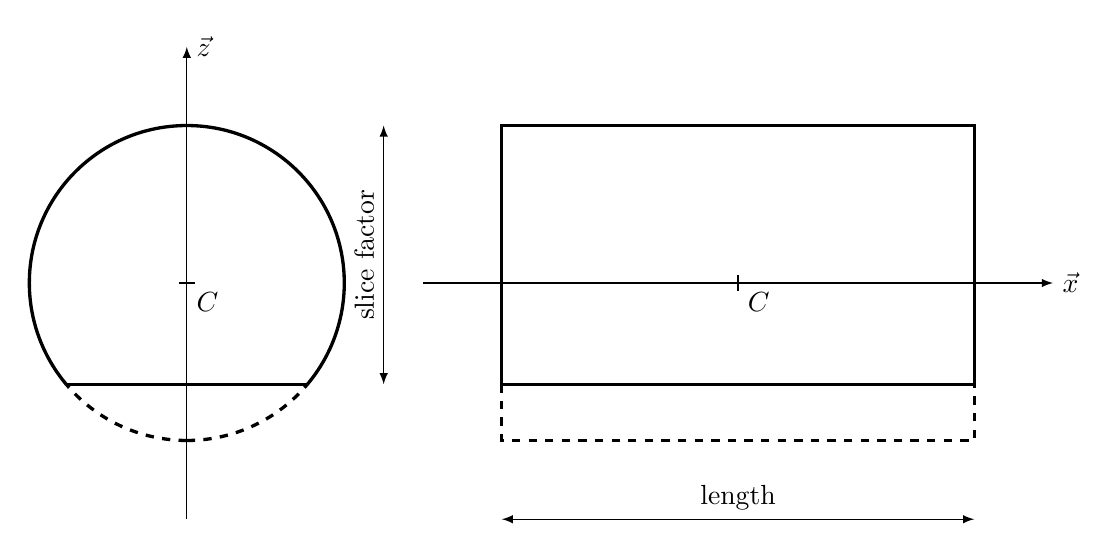
\begin{tikzpicture}
\draw [-latex] (0,-3) -- (0,3);
\draw (0,3) node[right]{$\vec{z}$};
\draw [-] (-0.1,0) -- (0.1,0);
\draw (0,0) node[below right]{$C$};

\draw [very thick,-](0,2) arc [start angle=90, end angle=220, radius=2];
\draw [very thick,-](0,2) arc [start angle=90, end angle=-40, radius=2];
\draw [very thick,dashed](0,-2) arc [start angle=-90, end angle=-140, radius=2];
\draw [very thick,dashed](0,-2) arc [start angle=-90, end angle=-40, radius=2];
\draw [very thick,-] (-1.5321,-1.2856) -- (1.5321,-1.2856);

\draw [latex-latex] (2.5,-1.2856) -- (2.5,2) node [midway,above,sloped] {slice factor};

\draw [-latex] (3,0) -- (11,0);
\draw (11,0) node[right]{$\vec{x}$};
\draw [very thick] (4,-1.2856) rectangle (10,2);
\draw [very thick,dashed] (4,-1.2856) -- (4,-2) -- (10,-2) -- (10,-1.2856);
\draw [-] (7,-0.1) -- (7,0.1);
\draw (7,0) node[below right]{$C$};
\draw [latex-latex] (4,-3) -- (10,-3) node [above,midway] {length};
\end{tikzpicture}\end{center}

The anchor points are
\begin{itemize}
	\item \textbf{SEL\_OBJ\_CYL\_CENTER} : the cylinder center
	\item \textbf{SEL\_OBJ\_CYL\_FACE\_XM} : the center of the face first intersecting the $x$ axis
	\item \textbf{SEL\_OBJ\_CYL\_FACE\_XP} : the center of the face last intersecting the $x$ axis
\end{itemize}

\newpage
\subsubsection{Lens}

While lenses could be defined from a sequence of spherical patches, a volume lens primitive is provided through the function \lfc{Selene\_object}(\lsg{lens},\lft{thickness},\lft{radius},\lft{$r_1$},\lft{$r_2$}).

A lens is made of two spherical caps and one cylinder. \lft{thickness} specifies the intersection points of each cap with the $\vec x$ axis of the lens, the first one being at -\lft{thickness}/2 and the second at \lft{thickness}/2. \lft{$r_1$} and \lft{$r_2$} are the radii of each, and \lft{radius} is the maxiùam radius of the lens from its axis.
\begin{center}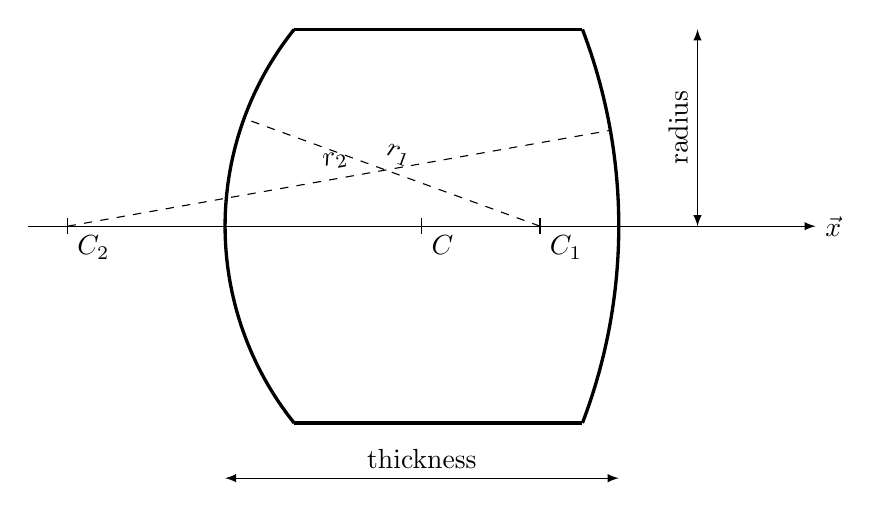
\begin{tikzpicture}
\draw [-latex] (-5,0) -- (5,0);
\draw (5,0) node[right]{$\vec{x}$};
\draw [-] (0,-0.1) -- (0,0.1);
\draw (0,0) node[below right]{$C$};

\draw [very thick,-](-2.5,0) arc [start angle=180, end angle=141.32, radius=4];
\draw [very thick,-](-2.5,0) arc [start angle=180, end angle=218.68, radius=4];
\draw [dashed] (1.5,0) -- (-2.2588,1.3681) node [midway,above,sloped] {$r_1$};
\draw [-] (1.5,-0.1) -- (1.5,0.1);
\draw (1.5,0) node[below right]{$C_1$};

\draw [very thick,-](2.5,0) arc [start angle=0, end angle=20.92, radius=7];
\draw [very thick,-](2.5,0) arc [start angle=0, end angle=-20.92, radius=7];
\draw [dashed] (-4.5,0) -- (2.3837,1.2155) node [midway,above,sloped] {$r_2$};
\draw [-] (-4.5,-0.1) -- (-4.5,0.1);
\draw (-4.5,0) node[below right]{$C_2$};

\draw [very thick,-] (-1.62235,2.5) -- (2.0383,2.5);
\draw [very thick,-] (-1.62235,-2.5) -- (2.0383,-2.5);

\draw [latex-latex] (-2.5,-3.2) -- (2.5,-3.2) node [midway,above] {thickness};

\draw [latex-latex] (3.5,0) -- (3.5,2.5) node [midway,above,sloped] {radius};
\end{tikzpicture}\end{center}
The faces of the lens are ordered as such:
\begin{enumerate}
	\setcounter{enumi}{-1}
	\item the spherical cap that first intersects the $x$ axis
	\item the second spherical cap
	\item the surrounding cylinder
\end{enumerate}
The lens anchors are
\begin{itemize}
	\item \textbf{SEL\_OBJ\_LENS\_CENTER}
	\item \textbf{SEL\_OBJ\_LENS\_FRONT}
	\item \textbf{SEL\_OBJ\_LENS\_REAR}
%	\item \textbf{SEL\_OBJ\_LENS\_F1}
%	\item \textbf{SEL\_OBJ\_LENS\_F2}
%	\item \textbf{SEL\_OBJ\_LENS\_P1}
%	\item \textbf{SEL\_OBJ\_LENS\_P2}
\end{itemize}

\newpage
\subsubsection{Prism}

\newpage
\subsubsection{Sphere}

Spheres are a primitive created through \lfc{Selene\_object}(\lsg{sphere},\lft{radius},\lft{slice factor}), where \lft{radius} is obviously the sphere radius.

Making hemispheres and every other similar shapes is the purpose of the \lft{slice factor}. Just like for cylinders, a value of 1 will give a full sphere, and a value of 0.5 will result into an hemisphere.
\begin{center}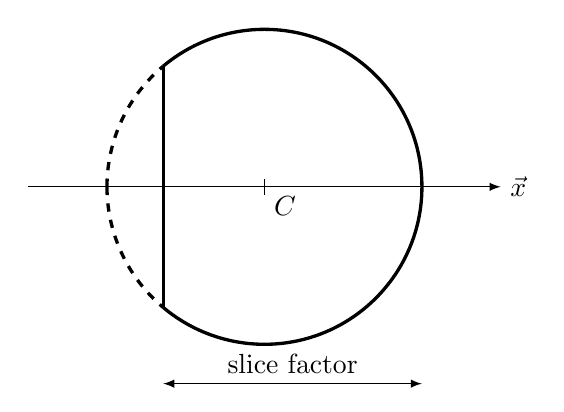
\begin{tikzpicture}
\draw [-latex] (-3,0) -- (3,0);
\draw (3,0) node[right]{$\vec{x}$};
\draw [-] (0,-0.1) -- (0,0.1);
\draw (0,0) node[below right]{$C$};

\draw [very thick,-](2,0) arc [start angle=0, end angle=130, radius=2];
\draw [very thick,-](2,0) arc [start angle=0, end angle=-130, radius=2];
\draw [very thick,dashed](-2,0) arc [start angle=180, end angle=130, radius=2];
\draw [very thick,dashed](-2,0) arc [start angle=180, end angle=230, radius=2];
\draw [very thick,-] (-1.2856,-1.5321) -- (-1.2856,1.5321);

\draw [latex-latex] (-1.2856,-2.5) -- (2,-2.5) node [midway,above] {slice factor};
\end{tikzpicture}\end{center}
There are two faces only to this object:
\begin{enumerate}
\setcounter{enumi}{-1}
	\item the spherical interface
	\item the flat face
\end{enumerate}
and two associated anchor points:
\begin{itemize}
	\item \textbf{SEL\_OBJ\_SPHERE\_CENTER}: the center of the sphere
	\item \textbf{SEL\_OBJ\_SPHERE\_SLICE\_CENTER}: the center of the flat face
\end{itemize}

\newpage
\subsection{Surface Primitives}

\subsubsection{Cylindrical surface}

\newpage
\subsubsection{Conical surface}

\newpage
\subsubsection{Disk}

Disks are flat surfaces that can help make diaphragms, and are added through \lfc{Selene\_object}(\lsg{disk},\lft{$r$},\lft{$r_{in}$}). The outer radius is defined by \lft{$r$}, and inner radius by \lft{$r_{in}$}. The disk extends in the $(y,z)$ plane, and its normal vector is pointed towards $-\vec x$.

Its only notable point is \textbf{SEL\_OBJ\_CENTER}.

\newpage
\subsubsection{Parabola}

Parabolas are basic optical surfaces that can be used to design aspheric lenses or parabolic mirrors. they can be added to a scene through \lfc{Selene\_object}(\lsg{parabola},\lft{focal},\lft{$r_{in}$},\lft{length}), with \lft{focal} the location of the focal point with respect to the apex and \lft{length} the total length of the parabola. The radius parameter \lft{$r_{in}$} is there to provide an easy way to open an aperture around the parabola tip.
\begin{center}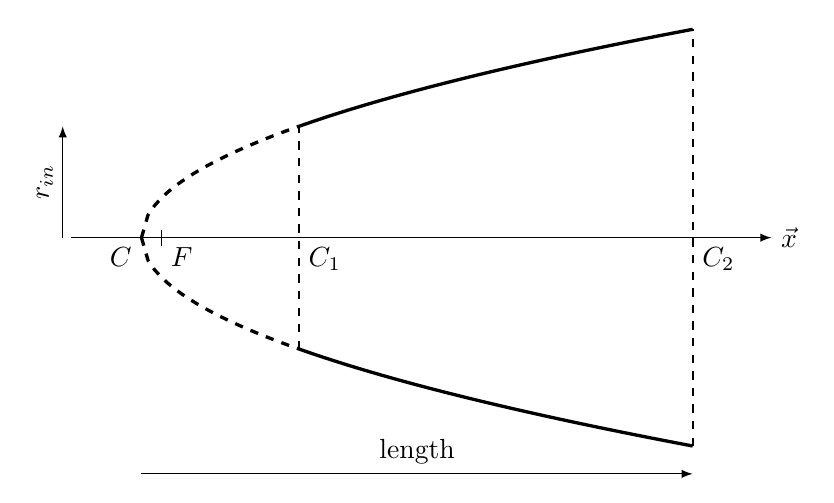
\begin{tikzpicture}
\draw [very thick,domain=0:2,dashed] plot (\x,{sqrt(\x)});
\draw [very thick,domain=2:7] plot (\x,{sqrt(\x)});
\draw [very thick,domain=0:2,dashed] plot (\x,{-sqrt(\x)});
\draw [very thick,domain=2:7] plot (\x,{-sqrt(\x)});
\draw [thick,dashed] (2,-1.4142) -- (2,1.4142);
\draw (2,0) node[below right]{$C_1$};
\draw [thick,dashed] (7,-2.6458) -- (7,2.6458);
\draw (7,0) node[below right]{$C_2$};
\draw [-] (-0.1,0) -- (0.1,0);
\draw (0,0) node[below left]{$C$};

\draw [-] (0.25,-0.1) -- (0.25,0.1);
\draw (0.25,0) node[below right]{$F$};

\draw [-latex] (-1,0) -- (-1,1.4142) node [midway,above,sloped] {$r_{in}$};

\draw [-latex] (0,-3) -- (7,-3) node [midway,above] {length};

\draw [-latex] (-0.9,0) -- (8,0);
\draw (8,0) node[right]{$\vec{x}$};
\end{tikzpicture}\end{center}
There is only one face to it, and its normal vector points outwards. There are, however, four notable points that can serve as anchors:
\begin{itemize}
	\item \textbf{SEL\_PARABOLA\_CENTER}: the tip of the parabola if it were full, noted by $C$ on the diagram above
	\item \textbf{SEL\_PARABOLA\_FOCUS}: the focal point of the parabola
	\item \textbf{SEL\_PARABOLA\_IN\_CENTER}: the center of the disk formed by the small aperture, noted $C_1$ above
	\item \textbf{SEL\_PARABOLA\_OUT\_CENTER}: the center of the disk formed by the end of the parabola, noted $C_2$ above
\end{itemize}

\newpage
\subsubsection{Rectangle}

The rectangle is the flat equivalent of the box. Is this created through \lfc{Selene\_object}(\lsg{rectangle},\lft{ly},\lft{lz}). It extends in the $(y,z)$ plane from -\lft{ly}/2 to +\lft{ly}/2, and -\lft{lz}/2 to +\lft{lz}/2.

The normal vector of the face is directed towards $-\vec x$. The only admissible anchor point is \textbf{SEL\_OBJ\_CENTER}.

\newpage
\subsubsection{Spherical patch}

\begin{itemize}
	\item \textbf{SEL\_OBJ\_SPHERE\_PATCH\_CENTER}
	\item \textbf{SEL\_OBJ\_SPHERE\_PATCH\_SLICE\_CENTER}
\end{itemize}

\subsection{Meshes}

This object type has access to specific functions
\begin{itemize}
	\item \lfc{add\_mesh}(\lsg{file\_name}): appends the mesh designed by \lsgnq{file\_name} to the object's mesh
	\item \lfc{auto\_recalc\_normals}(): recompute the face normals so that they all point outside
	\item \lfc{N\_faces}(): returns the total number of faces of the mesh
\end{itemize}

\subsubsection{Faces groups}

\lfc{define\_faces\_group}(\lin{group number},\lin{first face},\lin{last face})

\begin{itemize}
	\item \lfc{faces\_group\_down\_IRF}(\lin{group number},\lud{IRF})
	\item \lfc{faces\_group\_down\_mat}(\lin{group number},\lud{Material})
	\item \lfc{faces\_group\_down\_tangent}(\lin{group number},\lsg{type})
	\item \lfc{faces\_group\_down\_tangent}(\lin{group number},\lft{x},\lft{y},\lft{z})
	\item \lfc{faces\_group\_IRF}(\lin{group number},\lud{IRF})
	\item \lfc{faces\_group\_up\_IRF}(\lin{group number},\lud{IRF})
	\item \lfc{faces\_group\_up\_mat}(\lin{group number},\lud{Material})
	\item \lfc{faces\_group\_up\_tangent}(\lin{group number},\lsg{type})
	\item \lfc{faces\_group\_up\_tangent}(\lin{group number},\lft{x},\lft{y},\lft{z})
\end{itemize}

\subsection{Composite objects}

\subsubsection{Booleans}

\subsubsection{Composites}

\newpage
\section{Sensors}

\label{selene_sensors}
There would be not much point to a simulation software if one could do no analysis thanks to it. As such, some kind of sensors are necessary. In Selene, sensors are objects marked as such.

This is done through the \lfc{sensor} function, of which the first parameter specifies what kind of sensor. The following parameters specify what the sensor needs to record. Example:
\begin{lstlisting}
obj:sensor("abs","wavelength","ID","obj_intersection")
\end{lstlisting}

\subsection{Absorbing sensors}

This kind of sensor is basically a screen. Rays interacting with it are absorbed and disappear from the simulation. Absorbing sensors are specified with the \lsg{abs} parameter.

\subsection{Transparent sensors}

Object defined as transparent sensors behave according to their geometry, materials, IRFs, etc, but record interactions with rays. They can be used to monitor flux through a surface, or evaluate the number of rays that will be absorbed through a specific region of space. They are specified with the \lsg{transp} parameter.

\subsection{Recording options}

\begin{itemize}
	\item \lsg{wavelength}: records the ray wavelength
	\item \lsg{source}: records the ID of the source that generated the ray
	\item \lsg{path}: records the ray path ID. It is assigned by the source at generation, and can thus be common to several rays. It is unique for a single source.
	\item \lsg{generation}: records the ray number within a path, starting from 0, and increasing after each interaction
	\item \lsg{length}: records the ray optical path length at the intersection point
	\item \lsg{phase}: records the phase of the ray at the intersection point
	\item \lsg{world\_intersection}: records the coordinates of the intersection with respect to the scene frame
	\item \lsg{world\_direction}: records the directoin of the ray at the intersection with respect to the scene frame
	\item \lsg{obj\_intersection}: records the coordinates of the intersection with respect to the object frame
	\item \lsg{obj\_direction}: records the directoin of the ray at the intersection with respect to the object frame
\end{itemize}

\subsection{File format}

Objects marked as sensors will generate a file with a name like \lsgnq{object\_name\_ray\_sensor}.

The first line contains in the following order: the coordinates of the object center (three numbers), the vectors of the object frame (nine numbers), and the bounding box in the object frame. All those follow the $x$, $y$, $z$ order.

The second line is a string sequence that lists all the recorded options names.

Each subsequent line will correspond to an interaction containing the requested data in the order specified by the second line.

\newpage
\section{Sources}

Sources are what generate rays for the renderer to compute, and nothing would happen without them. They share many common functions with objects, but have a few dedicated ones. Source are created using the \lfc{Selene\_light}(\lsg{type},\lud{options...}) function. For instance
\begin{lstlisting}
light_1=Selene_light("point_planar")
\end{lstlisting}
will create a planar point source.

\subsection{Functions common to all light sources}

\label{selene_source_funcs}

\subsubsection[discrete\_spectrum]{\lfc{discrete\_spectrum}(\{\lft{lambda 1},\lft{lambda 2},\lft{...}\},\{\lft{weight 1},\lft{weight 2},\lft{...}\})}

Gives the source a discrete spectrum from a list of wavelength in meters, with their associated wavelengths
\begin{lstlisting}
light:discrete_spectrum({400e-9,500e-9,600e-9},{1,2,1.5})
\end{lstlisting}

\subsubsection[material]{\lfc{material}(\lud{Material})}

Sets the ambient material of the source to \lud{Material}.
\begin{lstlisting}
light:material(Glass)
\end{lstlisting}

\subsubsection[location]{\lfc{location}(\lft{x},\lft{y},\lft{z})}

Sets the source location to (\lft{x},\lft{y},\lft{z}) within the translation frame. The true location will be defined according to the relative positioning system. See \ref{selene_relative_positioning} for a detailled explanation.
\begin{lstlisting}
light:location(1,1,0)
\end{lstlisting}

\subsubsection[name]{\lfc{name}(\lsg{source name})}

Sets the source name to \lsgnq{name}.
\begin{lstlisting}
light:name("laser")
\end{lstlisting}

%\subsubsection[origin]{\lfc{origin}(\lsgnq{anchor name})}
%
%Sets the origin of the source to its anchor defined by \lsgnq{anchor name}. See \ref{selene_relative_positioning} for more details, and the sources descriptions for a list of the anchors.
%\begin{lstlisting}
%light:origin(SEL_LIGHT_BEAM_WAIST)
%\end{lstlisting}

\subsubsection[polar\_along]{\lfc{polar\_along}(\lft{x},\lft{y},\lft{z})}

Defines the axis vector (\lft{x},\lft{y},\lft{z}) along which the source will try to orient the polarization as close as possible. The sign of the whole vector is of no importance.
\begin{lstlisting}
light:polar_along(1,1,0)
\end{lstlisting}

\subsubsection[polar\_not]{\lfc{polar\_not}(\lft{x},\lft{y},\lft{z})}

Defines the axis vector (\lft{x},\lft{y},\lft{z}) that the source will try to avoid for rays polarization as much as possible. The sign of the whole vector is of no importance.
\begin{lstlisting}
light:polar_not(0,0,1)
\end{lstlisting}

\subsubsection[polar\_unset]{\lfc{polar\_unset}()}

Leaves to the source the choice of the polarization vector for each ray.
\begin{lstlisting}
light:polar_unset()
\end{lstlisting}

\subsubsection[power]{\lfc{power}(\lft{value})}

Sets the power of the source to anchor of the specified \lft{value} in Watts.
\begin{lstlisting}
light:power(55)
\end{lstlisting}

\subsubsection[relative\_origin]{\lfc{relative\_origin}(\lud{relative frame},\lsgnq{anchor name})}

Sets the relative origin of the source to anchor of the \lud{relative frame} designed by \lsgnq{anchor name}. See \ref{selene_relative_positioning} for more details, and the objects and sources descriptions for a list of the anchors.
\begin{lstlisting}
light:relative_origin(object_0,SEL_OBJ_BOX_FACE_XM)
\end{lstlisting}

\subsubsection[rotation]{\lfc{rotation}(\lft{$\alpha$},\lft{$\beta$},\lft{$\gamma$})}

Set the angles of rotation of the source to \lft{$\alpha$}, \lft{$\beta$} and \lft{$\gamma$}, in degrees, relative to the \lud{rotation frame}. See \ref{selene_relative_positioning} for more details.
\begin{lstlisting}
light:rotation(0,0,90)
\end{lstlisting}

\subsubsection[rotation\_frame]{\lfc{rotation\_frame}(\lud{frame})}

Set the relative rotation frame of the source the to one held by \lud{frame}. See \ref{selene_relative_positioning} for more details.
\begin{lstlisting}
light:rotation_frame(object_1)
\end{lstlisting}

\subsubsection[spectrum]{\lfc{spectrum}(\lsg{spectrum shape},\lud{option})}

Defines the source as a broadband source with the related \lsgnq{spectrum shape}. It can have three different values, with associated options.
\begin{itemize}
	\item \lfc{spectrum}(\lsg{flat},\lft{lambda min},\lft{lambda max}) will give the source a flat spectral flux between both boundaries, in meters
	\item \lfc{spectrum}(\lsg{file},\lsg{file\_name}) will load the associated file and assign it as the spectral flux of the source
	\item \lfc{spectrum}(\lsg{planck},\lft{lambda min},\lft{lambda max},\lft{temperature}) will define the source as a black body with the associated temperature in Kelvin, that will be sampled between the boundaries in meters
\end{itemize}

\subsubsection[translation\_frame]{\lfc{translation\_frame}(\lud{frame})}

Set the relative translation frame of the source to the one held by \lud{frame}. See \ref{selene_relative_positioning} for more details.
\begin{lstlisting}
light:translation_frame(lens)
\end{lstlisting}

\subsubsection[wavelength]{\lfc{wavelength}(\lft{lambda})}

Defines the source as a monochromatic source of wavelength \lft{lambda}, in meters.
\begin{lstlisting}
light:wavelength(533e-9)
\end{lstlisting}

\subsection{Source types}

\subsubsection{Perfect beam}

This source aims to represent a source place at infinity. Its rays are strictly parallel, along the $x$ axis of the source. It is instanced by the \lsg{perfect\_beam} parameter.

The function \lfc{aperture}(\lft{radius}) will set the size of the disk emitting the rays with the corresponding \lft{radius}, in meters.

\noindent Example:
\begin{lstlisting}
light=Selene_light("perfect_beam")
light:aperture(5e-3)
\end{lstlisting}

\subsubsection{Planar point source}

This source is similar to the point source, except it will emit in its $(y,z)$ plane only. A rotation by $\gamma=90^\circ$ is thus necessary to target the $(x,y)$ plane. It is created through the \lsg{point\_planar} parameter.\\ Example:
\begin{lstlisting}
light=Selene_light("point_planar")
\end{lstlisting}

\subsubsection{Point source}

This is the most basic source. It will emit in all directions homogeneously. It is created through the \lsg{point} parameter.\\ Example:
\begin{lstlisting}
light=Selene_light("point")
\end{lstlisting}

\subsection{Spectra}

To different types of analysis will correspond different input spectra. We provide a few ways of handling them.

In order to easily match the CIE illuminants, we assume all the spectra are actually spectral power distributions, in $W\cdot m^{-1}$, although this does not define the actual power of the source.

\subsubsection{Monochromatic sources}

Those are the most basic types of spectra. Every ray generated by those sources will be assigned the wavelength defined by \lfc{wavelength}.

\subsubsection{Poly-monochromatic sources}

They are the bridge between monochromatic sources and truly polychromatic sources, and can approximate lights with a small number of emission rays.

They are basically several monochromatic sources bundled into one, but with different weights associated with each wavelengths. Those wavelengths are then probabilistically given to the generated rays according to those weights.

Such spectra are assigned through the \lfc{discrete\_spectrum} function.

\subsubsection{Polychromatic sources}

Those are the truly polychromatic sources. In this, the spectrum is a continuous function going from $\lambda_{min}$ to $\lambda_{max}$. Wavelengths are then assigned to generated rays thanks to a rejection algorithm between those boundaries. We provide three types of polychromatic spectra
\begin{description}
	\item[Flat]: every wavelength between $\lambda_{min}$ and $\lambda_{max}$ is equiprobable
	\item[Planck]: the probability distribution here is the black body distribution in wavelength form
	\begin{equation}
		P(\lambda,T)=\frac{2*h*c^3}{\lambda^5}\frac{1}{e^{\dse -\frac{hc}{\lambda k_B T}}-1}
	\end{equation}
	\item[User defined]: in this case, the user provides a two columns text file, the first being the wavelength, and the second the associated probability. Wavelengths are then drawn to match this probability distribution
\end{description}

\subsection{Power normalization, spectra and rays}

\subsubsection{Time}

Time is an undefined quantity with respect to raytracing. One can could assume all the paths are computed exactly at the same time, or spread across several seconds. For convenience, it was decided computations would occur within one second, so that the values of power and total energy emitted could be treated as the same.

\subsubsection{Energy}

Generally, rays can not represent real photons due to the sheer number of those cast by a real light source. For instance, a 1W source would emit in the order of $10^{20}$ photons per second, and computing them all would require incredible computational power.

The issue is then figuring out how to represent those photons with far fewer of them, in particular the energy they carry. Real photons energy is wavelength dependent, with $E=hc/\lambda$, but using this is not particularly convenient.

For instance, let us assume we want to simulate a light source with a flat power spectrum: using the previous definition would imply that for one blue ray emitted by the source, there would be two red ones. Since the computation spatial accuracy is a factor of the number of rays cast, it would be twice as good for red ones than blue ones, which is leads to an imbalance in simulation results.

As such, it was decided that, by default, all rays should carry the same number amount of energy.

\subsubsection{Number of rays per source}

The total number of photons is set by the user, and they need to be distributed among sources. This is done thanks to the \lfc{power} function which is serves both to relate sources to eachother, and to define how much energy rays will carry.

If each source $i$ emits a power $P_i$, and the total number of photons is $N$, then the number of rays per source $N_i$ will be
\begin{equation}
	N_i=N\frac{P_i}{\dse \sum_i P_i}
\end{equation}
and the power of each ray will be
\begin{equation}
	P_r=\frac{1}{N} \sum_i P_i
\end{equation}

\chapter{Selene: GUI}

The purpose of this chapter is to explain the graphical interface used to manipulate Selene. In most aspects, it is a direct translation of the scripting interface into a GUI.

As such, it is highly advised to read the previous chapter containing all the fine details about the working principles, the constants related to the renderer or objects, etc.

\section{Main window}

Selene's GUI is initiated by clicking the Selene button on the startup window. The window that opens is separated into four main parts: the display panel, the rays display options, the scene tree and the rendering options.

\subsection{3D display}

\subsection{Rays Display}

\subsection{Scene tree}

The scene tree summarizes the objects and light sources included in the scene. It is also the control that will serve to add new elements, modify or delete them. Elements that have a relative origin will appear as leaves of the related element.

\subsubsection{Adding a new element}

At the top of the scene tree sits a drop-down list that contains all the elements that can be added. Those are both objects and sources. Adding a new element first requires selecting the relevant element, and then clicking the \lfc{Add} button.

The related element dialog with all its parameters will then open, but the element will only be added after clicking the \lfc{Ok} button. The addition will be cancelled otherwise.

\subsubsection{Modifying an element}

Elements belonging to the tree can be modified by a right click on them. This brings a popup menu up with two choices
\begin{itemize}
	\item \lfc{Properties} shows the element dialog that allows one to modify the various properties
	\item \lfc{Delete} will remove the element from the scene. In the case it were used as a relative frame for any other element, the latter will have said frame invalidated
\end{itemize}

\subsection{Rendering}

Once a scene is complete and properly set up (and saved to a file to avoid any lost work), rendering it is the final step. The controls related to it will be found at the bottom left of the window. It contains three parts:
\begin{itemize}
	\item The \lfc{N Disp} control will define how many paths to display at most in the 3D view
	\item The \lfc{N Tot} control defines how many initial rays to cast from the sources.
	\item The \lfc{Trace} button will render the scene.
\end{itemize}
After the computation is over, the 3D display will show a subset of the rays that have been computed for immediate feedback, and the various sensors will have their files written to the hard drive.

\section{The object dialog}

The object dialog is split into four parts, three of them being tabs:
\begin{itemize}
	\item the controls panel on the left is always visible. It serves to control the object name, and the various properties of the positioning system. Those are then followed by the specific object properties.
	\item the \lfc{Geometry} tab shows a 3D view of the object geometry, according to the object properties
	\item the \lfc{Interfaces} tab serves to control the properties of each face: materials, IRFs and tangent vectors
	\item the \lfc{Sensor} tab helps defining if an object is a sensor, what kind and what it should record
\end{itemize}

\section{The light source dialog}

The source dialog is split into two parts
\begin{itemize}
	\item the controls panel on the left is always visible. It serves to control the source name, and the various properties of the positioning system. Those are then followed by the specific source properties.
	\item the \lfc{Spectrum} tab serves to define the source spectral properties. Its layout changes depending on the kind of spectrum selected
\end{itemize}

\section{The materials dialog}

%%%%%%%%%%%%%%%%%%%%%%%%%%%%
%   Multilayer structures
%%%%%%%%%%%%%%%%%%%%%%%%%%%%

\part{Multilayers}

\chapter{Multilayers optical response: scripting interface}

\section{Basic setup}

\lfc{spectrum}

\lfc{output}

\section{Structure definition}



\subsection{Environment}

\lfc{substrate}

\lfc{superstrate}

\subsection{Layers}

\lfc{add\_layer}

\section{Optical response computation}

\lfc{compute\_angle}

\section{Guided modes computation}

\lfc{compute\_guided}


\chapter{Multilayers optical response: GUI}

The GUI version of Aether contains a tool dedicated to computing the optical response of multilayer structures. This is accessed from the startup window through the \lfc{Multilayers} button.

\section{Computation modes}

The tool is split into two modes: spectral and angular. Both requires setting up a few controls. First, the spectrum is set with \lfc{Lambda min} and \lfc{Lambda max}, containing \lfc{N Points}. The angles of incidence are assumed to go from 0$\deg$ to 90$\deg$ with \lfc{N Angles} points.

\subsection{Spectral mode}

In the spectral mode, the results will computed with respect to the spectrum, and the user will browse through the angles thanks to the slider below the graph. The slider will go from 0$\deg$ to 90$\deg$ with \lfc{N Angles}.

\subsection{Angular mode}

In the angular mode, the results will computed with respect to the angle of incidence, and the user will browse through the spectrum from \lfc{Lambda min} to \lfc{Lambda max} thanks to the slider with \lfc{N Points} increments.

\section{Multilayer structure definition}

First the materials of the substrate and superstrate need to be defined. This is done through the \lfc{Superstrate} and \lfc{Substrate} material selectors. Note that
\begin{itemize}
	\item the incident light is assumed to be coming from the superstrate
	\item as such, the refractive index of the superstrate can only be real
	\item the angle of incidence is defined inside the superstrate
\end{itemize}
Once this is done, the various layers must be added. This is done by first selecting the layer type from the drop-down list, and then clicking \lfc{Add}, within the \lfc{Layers} control.

\subsection{Layer}



\subsection{Bragg structure}

For convenience, the possibility of creating Bragg structures has been added.

\subsection{Statistical thickness distribution}

If one wants 

The total number of samples is selected from the \lfc{Statistical Sampling} control. 

\section{Results}

The results are shown in real-time on the on the right of the window. There are nine curves in total:
\begin{itemize}
	\item the reflection, transmission and absorption for the S polarization (TE)
	\item the reflection, transmission and absorption for the P polarization (TM)
	\item the averages of both sets of curves
\end{itemize}
Their display can be selectively enabled or disabled thanks to the checkboxes under \lfc{Display}.

\section{Exporting the result}

The data shown on the graph can be exported through the \lfc{Export Data} button.

\chapter{Guided modes calculation: GUI}

%%%%%%%%%%%%%%%%%
%   Misc stuff
%%%%%%%%%%%%%%%%%

\part{Various tools}

\chapter{Scripting tools}

\section{dielec\_planar\_waveguide}

%	Ce mode permet de calculer rapidement les indices effectifs des modes guidés d'un guide plan diélectrique. Les différents indices sont définis par les fonctions \lfc{guide}(\lft{index}), \lfc{superstrate}(\lft{index}) et \lfc{substrate}(\lft{index}). L'épaisseur du guide est définie par \lfc{thickness}(\lft{h}) tandis que la longueur d'onde à étudier est donnée grâce à \lfc{lambda}(\lft{$\lambda$}).
%	
%	Les résultats s'affichent immédiatement à l'écran et s'accumulent dans le fichier \lsgnq{modes.txt}.

\fwarn

\begin{lstlisting}
guide=MODE("dielec_planar_waveguide")
guide:guide(1.9)
guide:substrate(1.0)
guide:superstrate(1.1)
guide:thickness(200e-9)
guide:lambda(500e-9)
\end{lstlisting}

\section{fieldblock\_treat}

\section{fieldmap\_treat}

\section{index\_fit}

\section{preview\_fdtd\_structure}

This mode allows to load and visualize a FDTD geometry file (c.f. chapter \ref{geomsection}) without requiring a simulation to be launched. Only the \lfc{structure}(\lsg{geometry\_file}) function is available in this mode. The result is displayed in the \lsgnq{grid} directory.\\ Example:
\begin{lstlisting}
test=MODE("preview_fdtd_structure")
test:file("structures/nanorods_grid.lua")
\end{lstlisting}

\chapter{Diffraction orders}

The purpose of this tool is to help understand the number of propagative diffraction orders that can exist in the optical response of a flat diffraction grating. It's split in two modes selected thanks to the \lfc{Mode} switch.

It is accessed through the \lfc{Diffraction Orders} button in the startup window.

\section{Monochromatic mode}

This is the most graphically interesting mode. The window is split in two parts: the controls on the left, and the 2D view on the right. The controls are as follows:
\begin{itemize}
	\item the \lfc{Lambda} selector defines the wavelength of interest
	\item \lfc{Substrate} and \lfc{Superstrate} define the refractive index of either side of the grating. Note that \textcolor{red}{only real refractive indexes must be used}
	\item the \lfc{Incidence} of the incoming light is set through \lfc{Theta}, which is the angle from the normal vector, and \lfc{Phi} which is the azimuth
	\item the grating parameters are set by defining the vectors of the elementary cell. This is done through the controls inside \lfc{Grating Vector 1} and \lfc{Grating Vector 2}, for which the \lfc{Length} can be modified, as well as their \lfc{Angle} from the $\vec x$ axis.
\end{itemize}
The 3D view, on the right, shows the propagation direction of the various orders: red for those propagating into the superstrate, and blue for those propagating into the substrate. The green ray is the incident ray.

Note that the behavior of the 3D view can be modified through the \lfc{Display} controls:
\begin{itemize}
	\item \lfc{Normalized} changes wether the rays have the same length, or are scaled like wave vectors.
	\item \lfc{Superstrate} enables or disables the superstrate rays.
	\item \lfc{Substrate} enables or disables the substrate rays.
\end{itemize}

\section{Polychromatic mode}

The polychromatic mode is similar to the monochromatic one, except for a few modifications.

The first one is, obviously, that the wavelength is replaced with a spectrum selector, that asks for a range between \lfc{Lambda min} and \lfc{Lambda max}, and a number of computed points \lfc{N Points}.

The second modification is that the 3D visualization is replaced with a graph. This graph counts the total number of propagative diffraction orders that are present either in the superstrate or in the substrate. Note that for the superstrate this number can only go down to 1, for specular reflection can always exist.

The final modification is the \lfc{Surface Modes} button. This brings a dialog up that summarizes the wavelengths for which new propagative orders appear. This computation is not exact, but based on the points of the defined spectrum. The purpose of this window is to have a guide to interpret experimental spectra, so perfect accuracy is not necessary, and can always be refined by increasing the number of points in the spectrum.

\chapter{Graphical functions fitter}

\section{Exporting the fit}

\chapter{Samples Explorer}

The aim of the samples explorer is to help navigate a large number of samples in a use friendly way, by dynamically generating an interface based on written rules for each sample.

\section{Working principle}

Let us assume we have a set of samples in a directory as shown in figure \ref{samples_explorer_directories}.

\def\step{0.5}
\newcommand{\dpoint}[2]{(#1*\step,-#2*\step)}
\newcommand{\dcorner}[4]{\draw [thick] \dpoint{#1}{#2} -- \dpoint{#1}{#4}; \draw [thick] \dpoint{#1}{#4} -- \dpoint{#3}{#4};}
\begin{figure}[!ht]
\begin{tikzpicture}
\draw (0,0) node[right]{Samples directory};
\dcorner{0}{0}{1}{1}
\draw \dpoint{1}{1} node[right]{Project A};
\dcorner{1}{1}{2}{2}
\draw \dpoint{2}{2} node[right,red]{Sample a};
\dcorner{1}{1}{2}{3}
\draw \dpoint{2}{3} node[right]{Subproject SA};
\dcorner{2}{3}{3}{4}
\draw \dpoint{3}{4} node[right,red]{Sample 1};
\dcorner{2}{3}{3}{5}
\draw \dpoint{3}{5} node[right,red]{Sample 2};
\dcorner{1}{1}{2}{6}
\draw \dpoint{2}{6} node[right]{Subproject SB};
\dcorner{2}{6}{3}{7}
\draw \dpoint{3}{7} node[right,red]{Sample 3};
\dcorner{0}{0}{1}{8}
\draw \dpoint{1}{8} node[right]{Misc Directory};
\dcorner{1}{8}{2}{9}
\draw \dpoint{2}{9} node[right]{Mic Subdirectory};
\dcorner{0}{0}{1}{10}
\draw \dpoint{1}{10} node[right]{Project B};
\dcorner{1}{10}{2}{11}
\draw \dpoint{2}{11} node[right,red]{Sample 3};
\dcorner{1}{10}{2}{12}
\draw \dpoint{2}{12} node[right,red]{Sample 4};
\end{tikzpicture}
\caption{Example of a directory tree for the samples explorer module}
\label{samples_explorer_directories}
\end{figure}
In this, the directories containing actual samples data are highlighted in red. The aim of the SE is to create a GUI that will display the chosen samples information and data, while ignoring the directories that do not have any.

To do so, the user will chose the root directory that is to be analyzed, and the program will traverse all the subdirectories looking for samples. Those are indicated by the presence of a \lsgnq{desription.txt} file inside each of them. Without one, the content of a directory will be ignored, and so will be any text file that does not match that exact file name.


\section{The description file}

As stated before, each directory of interest must contain a \lsgnq{description.txt} file. This file contains the elementary instructions that will generate the related sample user interface. Strictly speaking, it is a Lua script and will be used to call several functions.
\begin{itemize}
	\item \lfc{date}(\lsg{date in any format}) : will give a date to the sample. That date does not need to follow any particular format.
	\item \lfc{description}(\lsg{description text}) : adds a description to the sample. There is no size limit to it. New lines must be defined with a \textbackslash  n statement within the string.
	\item \lfc{tags}(\lsg{tag 1},\lsg{tag 2},\lsgnq{...}) : tags associated to the sample. They can be anything, usually project names, geometry, etc, and will be used for filtering (see \ref{samples_explorer_tags}).
	\item \lfc{add\_image}(\lsg{path}) : path to the image to display, this can be called several times to display several pictures onto the interface
	\item \lfc{image\_description}(\lsg{description text}) :  adds a description to the last image defined with \lfc{add\_image}
	\item \lfc{add\_graph}(\lsg{caption}) : defines a new graph with its associated caption
	\item \lfc{add\_data}(\lsg{first file path},\lin{column number of file 1},\lsg{second file path},\lin{column number of file 2}) : this will add data to be displayed onto the last defined graph. The data must come from text files that contains several columns. The first two arguments will define the abscissa, while the last two define the data values. Columns counting start at 0.
	 \item \lfc{axis}(\lft{x1},\lft{x2},\lft{y1},\lft{y2}) : will set the default display axis of the last defined graph
\end{itemize}
Using those functions is not mandatory, and they can be omitted if irrelevant. Here is an example of what such a file could look like:
\begin{lstlisting}
description("Sample 1")

tags("t1","t4")

add_image("im1.jpg")
image_description("First image")

add_image("im2.jpg")
image_description("Second image")

add_image("subdir/im3.jpg")

add_graph("Graph 1")
add_data("data1.txt",0,"data1.txt",1)
axis(0,10,-0.5,1.5)

add_graph("Graph 2")
add_data("data1.txt",0,"data1.txt",1)
add_data("data2.txt",0,"data2.txt",2)

add_graph("Graph 3")
add_data("data1.txt",0,"data1.txt",1)
add_data("data2.txt",0,"data2.txt",1)
add_data("data2.txt",0,"data2.txt",2)
\end{lstlisting}

\section{Interface}

Once the various samples have been put in their directories, and their description files written, using the module is fairly simple.

The very first step is to define the root directory of the samples. This is done through the \lfc{...} button within the \lfc{Directory} box. The dialog that appears will ask for the root directory.

Once set, the software browses all of the subdirectories looking for description files, and treats them. The processing can take some time depending on the number of samples. If all goes well, the interface should update in two ways:
\begin{itemize}
	\item the list on the left of the window should now be populated by a list of all the samples and their directories.
	\item the panel on the right should now contain an aggregate of all the samples, each having a sample panel.
\end{itemize}

\subsection{The sample panel}

Each sample panel contains the information specified in the associated description file. 

\subsection{Tags filtering}

\label{samples_explorer_tags}
Tags would be of little point if they could not be used to filter the results. This is the purpose of the \lfc{Filter Tags} button at the bottom left of the window. A dialog appears after clicking it, and it will help 


%\part{Appendix}
%
%\appendix
%
%\chapter{Technical specifications and design documents}

The purpose of this chapter is to regroup various conventions, for internal or external development purposes. For instance, file specifications will be described there.

\section{Field Block Files}

\section{Field Maps Files}

\section{Selene}


\bibliographystyle{unsrt}
\bibliography{c:/docu/master_biblio}

\end{document}